\documentclass[12pt,a4paper,oneside,openright]{book}
\renewcommand{\thesection}{\arabic{section}}
%\usepackage{hyperref} % per link nel documento 
\usepackage[T1]{fontenc}
\usepackage[english]{babel}
%\usepackage{biblatex}
\usepackage[numbers]{natbib}
\usepackage{amsmath}
\usepackage{amssymb}
\usepackage{amsthm}
\usepackage{mathtools}
\usepackage{graphicx} 
\usepackage{indentfirst} 
\usepackage{url}
\usepackage{fancyvrb} 
\usepackage{listings} 
\usepackage[]{fncychap}
\usepackage{amsfonts}
\usepackage[bf,small]{caption}
\usepackage{xcolor}
\usepackage{changebar}
\usepackage[ruled,linesnumbered]{algorithm2e}
\usepackage{lipsum}                     % Dummytext
\usepackage{xargs} 
\usepackage{bbm}
\usepackage{bbold}  
\usepackage[english]{babel}
\selectlanguage{english}
\usepackage{url}
\usepackage{lipsum}
\usepackage{amsfonts}
\usepackage{epstopdf}
%\usepackage{algorithm}
\usepackage{algcompatible}

%\usepackage{algorithmic}
\usepackage{enumitem}
\usepackage{bm} 
%\usepackage{float} se c'è algorithm questo non serve!
\usepackage{amsopn}
\usepackage{chngcntr}
\DeclareMathOperator{\diag}{diag}
\DeclareGraphicsExtensions{.eps,.pdf,.png,.jpg}
\newtheorem{theorem}{Theorem}
\counterwithin{figure}{section}
\counterwithin{table}{section}
\counterwithin{equation}{section}
\counterwithin{theorem}{section}
\newtheorem{lem}{Lemma}
\usepackage{xr}

\externaldocument{capitolo1}
\externaldocument{capitolo2}
\externaldocument{capitolo3}
\usepackage{tikz}
\usetikzlibrary{positioning,shapes,shadows,arrows}
\tikzset{
	% ->, >=stealth,
	% line width=2.75pt,
	every path/.style={->, >=stealth, very thick, rounded corners},
	state/.style={
		rectangle, rounded corners,
		draw=black, fill=gray!20, thick,
		minimum height=2em, inner sep=10pt, text centered
	}
}

                   % Use more than one optional parameter in a new commands
%\usepackage[pdftex,dvipsnames]{xcolor}  % Coloured text etc.
%\usepackage[colorinlistoftodos,prependcaption,textsize=tiny]{todonotes}
%\newcommandx{\unsure}[2][1=]{\todo[linecolor=red,backgroundcolor=red!25,bordercolor=red,#1]{#2}}
%\newcommandx{\change}[2][1=]{\todo[linecolor=blue,backgroundcolor=blue!25,bordercolor=blue,#1]{#2}}
%\newcommandx{\info}[2][1=]{\todo[linecolor=OliveGreen,backgroundcolor=OliveGreen!25,bordercolor=OliveGreen,#1]{#2}}
%\newcommandx{\improvement}[2][1=]{\todo[linecolor=Plum,backgroundcolor=Plum!25,bordercolor=Plum,#1]{#2}}



\hyphenation{a-gen-tiz-za-zio-ne}
\hyphenation{e-co-no-me-trics}
\hyphenation{mo-dels}

%\graphicspath{{immagini_multistato/}}
\pagestyle{plain}

\linespread{1.3}

\usepackage{listings}
\usepackage{color}

\definecolor{dkgreen}{rgb}{0,0.7,0}
\definecolor{gray}{rgb}{0.5,0.5,0.5}
\definecolor{mauve}{rgb}{0.58,0,0.82}

% set the default code style
\lstset{
	frame=tb, % draw a frame at the top and bottom of the code block
	tabsize=4, % tab space width
	showstringspaces=false, % don't mark spaces in strings
	numbers=left, % display line numbers on the left
	commentstyle=\color{dkgreen}, % comment color
	keywordstyle=\color{blue}, % keyword color
	stringstyle=\color{red} % string color
}

\renewcommand{\texttt}[1]{%
	\begingroup
	\ttfamily
	\begingroup\lccode`~=`/\lowercase{\endgroup\def~}{/\discretionary{}{}{}}%
	\begingroup\lccode`~=`[\lowercase{\endgroup\def~}{[\discretionary{}{}{}}%
	\begingroup\lccode`~=`.\lowercase{\endgroup\def~}{.\discretionary{}{}{}}%
	\catcode`/=\active\catcode`[=\active\catcode`.=\active
	\scantokens{#1\noexpand}%
	\endgroup
}
%\lstset{frame=tb,
%  language=Java,
%  aboveskip=3mm,
%  belowskip=3mm,
%  showstringspaces=false,
%  columns=flexible,
%  basicstyle={\small\ttfamily},
%  numbers=none,
%  numberstyle=\tiny\color{gray},
%  keywordstyle=\color{blue},
%  commentstyle=\color{dkgreen},
%  stringstyle=\color{mauve},
%  breaklines=true,
%  breakatwhitespace=true,
%  tabsize=3
%}


\begin{document}

\thispagestyle{empty}

\vspace*{-1.5cm} 
\begin{bfseries}

\begin{center}
	\Large
	POLITECNICO DI MILANO\\
	\Large
	School of Industrial Engineering and Information\\
	Master's Degree in Mathematical Engineering\\
	\begin{figure}[htbp]
		\begin{center}
			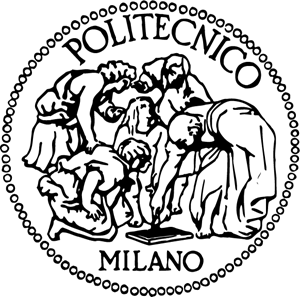
\includegraphics[width=4cm]{logopoli}
		\end{center}
	\end{figure}
	\vspace*{0.3cm} \LARGE		
	\textbf{A Scalable Positivity Preserving Solution Scheme for Coupled Nonlinear Advection-Diffusion-Reaction Problems}\\		
\end{center}
\vspace*{3.0cm}

\end{bfseries}

\vspace*{2cm}	
\begin{flushleft}
	\Large
	Supervisor: Prof. Carlo De Falco \\
\end{flushleft}
\vspace*{1.4cm}
	
\begin{flushright}
	\Large
	Candidate: Temenuzhak Valentinova AVRAMOVA\\
	Personal ID:  853568\\ 
\end{flushright}	
\vspace*{1.7cm}
	
\begin{center}		
	\Large
	Academic Year 2017-2018
\end{center} \clearpage










\frontmatter %----------------

\thispagestyle{empty}
%\include{dedica}

\tableofcontents 
% DA METTERE INDICE
\listoffigures
\listoftables

%\include{sommario}

\mainmatter %---------------

\chapter{Tumor growth's model}
\section{Propose of the thesis}
The main aim of our work is to propose a strategy to solve coupled nonlinear partial differential equations with constrained variables. Our attention will be focus on the main passages that are required for this kind of numerical solving, that are:
\begin{itemize}
	\item time discretization,
	\item space discretization,
	\item nonlinear method,
\end{itemize}  
where each point will be addressed in the next two chapters. \\
There are many examples of problems with the features that we nominated, for example Turing systems, generally nonlinear, with variables that represent chemical concentration of two species, therefor constrained to be nonnegative. \\
The example problem that we chose is taken from article "On interfaces between cell populations with different mobilities" \cite{tumor_growth}, because we know from previous studies on it, that it can be complicated enough to be a suitable test problem for validity and performances of our strategy.
Let see how it is structured. 
\section{Tumor growth}
\subsection {Introduction to the model}
We introduce a system of coupled time-depending advection-diffusion-reaction equations meat to describe the propagation of avascular tumor taken from \cite{tumor_growth}.
\begin{equation}
\label{tumor_system}
\begin{cases}
\partial_t m -\mu \; \nabla (m \nabla p) = G(p) m ,\\
\partial_t n -\nu \; \nabla (n \nabla p) = 0 .
\end{cases}
\end{equation}
Variable $ m $ indicates local density of \textit{dividing cells}, therefore those of the cancer, while $ n $ is local density of healthy cells, considered \textit{non-dividing }. Therefore both are constrained to be nonnegative. Pressure is given by a constitutive relation, in this way :
\begin{equation}
\label{pressure}
p := K_\gamma (n+m)^\gamma,
\end{equation}
with $ K_\gamma = \frac{\gamma + 1}{\gamma} $, where $ \gamma $ is a positive parameter that controls the stiffness of pressure law. Coefficients $ \mu > 0$ and $ \nu > 0 $ stand for mobility of dividing and non-dividing cells  respectively.\\
Second term of the left-hand-side model is a recall of the Dracy's law since is suggest the tendency of cells to move down the pressure gradient.\\
Right-hand-side of first equation indicates reasonably that growth of division cells $ m $ is proportional to its own density trough the quantity $ G(p) $. All this model is based on the observation that proliferating cells, $ m $, exert a pressure on their neighbours, $ n $,  and this result is a cell motion, that makes the first ones push forward the seconds. However, because of the competition fo space, when the pressure is above a threshold, that it is called \textit{homeostatic pressure} $ P_M $, then the system enters in a quiescent state. For all this reasons, it is required that $ G(P_M) = 0 $ and $ G'(p) < 0 $, because when pressure increases, so the competition of space, the devision rate has to decrease. \\
As announced in \cite{tumor_growth}, two cases has to be distinguished. When the dividing cells are more viscous ($ \nu > \mu $), so characterized by less mobility, than non-dividing ones, is supposed to generate segregation, that is $ m $ and $ n $ separated through a sharp interface.
Second case is the opposite one, $ \mu > \nu $, that corresponds to the situation in which "more viscous fluid" expands in a "less viscous" one. This scenario is expected to generate instabilities.\\
\subsection{One-dimensional traveling waves}
Suppose that we are looking fro solution of the form $ m(x,t) = m (x - \sigma  t) $ and $n(x,t) = n (x - \sigma  t)$, with $ \sigma $ traveling wave's velocity. Let start with an initial condition in which $ m $ and $ n $ lie on supports and are strictly separated, that is : $ Supp (m) = (-\infty, 0] $ and $ Supp (n) =  [0,r] $, with $ r = 1 $.\\
 Then \eqref{tumor_system} becomes:
\begin{equation}
\label{tumor_system_1d}
\begin{cases}
-\sigma m' - \mu (mp')' = G(p)m, \\
- \sigma n' - \nu (n p')' = 0
\end{cases}
\end{equation}
The reaction term is chosen in this way $ G(p) = P_M -p $. If we suppose that $ p' $ vanishes at $\pm \infty$, then from the second equation of \eqref{tumor_system_1d}, it is obtain:
\begin{equation}
\label{eqn}
(\sigma + \nu p')n = \sigma n_{\infty},
\end{equation}
where $ n \rightarrow n_{\infty} $ for $ x \rightarrow \infty $. In general we will take the case $ n_\infty = 0 $, consequently, from \eqref{eqn}, it comes:
\begin{equation}
\label{pn}
p_n(\xi) = \frac{\sigma}{\nu} (r - \xi),
\end{equation}
with $ \xi = x - \sigma t $ and $ x \in [0, r] $. Since $ m  $ is equal to 0 in the support of $ n $, using \eqref{pressure}, the solution of second equation in \eqref{tumor_system_1d} is :
\begin{equation*}
n(\xi) = \Big(\frac{p(\xi)}{K_\gamma} \Big)^\frac{1}{\gamma}.
\end{equation*}
While to find the solution of first equation in \eqref{tumor_system_1d}, we need to put ourselves in the case of large $ \gamma $ (incompressibility limit), that can be seen as  $ \gamma =  \frac{1}{\epsilon} $, with $ 0 < \epsilon << 1 $. Adding the equations of \eqref{tumor_system_1d}, it is obtained
\begin{equation}
\label{sum_eq}
-\sigma (m  + n)' - ((\mu m + \nu n)p')' = m G(p).
\end{equation} 
In particular, on the support of $ m $, it becomes: 
\begin{equation*}
-\sigma p ' - \mu (p'^2 + \gamma p p'') = \gamma p G(p).
\end{equation*}
We look for a solution of the following form: 
\begin{equation}
\label{pm}
p_m(\xi) = P_0(\xi) + \epsilon  P_1 (\xi),
\end{equation}
with $ p(-\infty) = P_M $.\\
Now, if we integrate \eqref{sum_eq}, it becomes : $ -\sigma (m + n) (x) - ((\mu m + \nu n) p')(x) = \int^{1}_{x} mG(p)$. By the continuity of $ m $, $ n $ and, consequently, of $ p $, and \eqref{pn}, this expression is obtained:
\begin{equation*}
p'(0^-) = \frac{\nu}{\mu} p'(0^+)=-\frac{\sigma}{\mu}.
\end{equation*} 
This is used as boundary condition for \eqref{pm}, then, if we neglect the part multiplied by $ \epsilon $, we obtain :
\begin{eqnarray}
\label{solpm}
p_m(\xi) = P_M + (\frac{\sigma}{\nu} - P_M) \exp \Big({\frac{\xi}{\sqrt{\mu}}}\Big), \; \; \; \text{with} \; \; \;
\sigma = \frac{P_M \sqrt(\mu) \nu}{r\sqrt{\mu} + \nu}.
\end{eqnarray}
The expression of $ p_m(\xi) $ and $ p_n(\xi) $ can be used as initial guess, putting $ \xi = x $, and then, a way to validate the chosen numerical method, is to verify if the wave's velocity, that we see in the simulations, is the theoretical one of \eqref{solpm}.
Theory of this section is taken from \cite{tumor_growth}, but there is also a contribution from professor Pasquale Ciarletta, that helped us finding the expression of the solution.\\
\subsection{Bi-dimensional propagation}
In paper \cite{tumor_growth} it is investigated also the behaviour of two-dimensional spherical waves with zero Neumann boundary conditions and initial conditions:
\begin{equation*}
m(x,y,t=0) := a_m e^{-b_m (x^2 + y^2)} \; \; \; \; \text{and}\; \; \; \; n(x,y,t=0) := a_n e^{-b_n (x^2 + y^2)} ,
\end{equation*}
with 
\begin{equation*}
a_m = 0.1, \; \; \; a_n =0.8, \; \;\; b_m = 5 \times 10^{-1}, \; \; \; b_n = 5 \times 10^{-7}.
\end{equation*}
Furthermore, reaction term is defined in the following way 
\begin{equation*}
G(p):= \frac{200}{\pi}\arctan(4(P_M-p))_+, \;\;\; P_M = 30,
\end{equation*}
with a domain of  $[0, L] \times [0, L]$, with $ L = 45 $.\\
We are going to test both one and bi-dimensional case, taking settings used by them as a first test, and then trying to stimulate the problem in different ways in order to test out strategy of solving. 
\chapter{Discretization of the problem}
\section{Time discretization}
Let consider a general differential equation in the following form: 
\begin{equation}
\label{diff_time}
u^\prime = f(t,u), \; \; \; \text{with} \; \;\; u(t_0) = u_0.
\end{equation} 
We can image this as a different way of writing a time depending partial differential equation, like those of our test problem \eqref{tumor_system} in the previous chapter. Indeed, $ u' $ represents $ \partial_t m $ or $ \partial_t n $, while $ f(t,u) $ contains all the rest of the equations. \\
One common way to discretize in time is to use Eulero's backward method, that consists in :
\begin{equation*}
u_{n+1} = u_n +  \Delta_n t \; f(t_{n+1}, u_{n+1}), \; \; \; \text{with}\; \; \; u_i := u(t_i)\; \;\; \text{and} \; \;\; \Delta_n t = t_{n+1}-t_n .
\end{equation*}
Actually this is what we want to use, but in general we know that its order of convergence is only 1. Therefore, we expect that, if we ask high accuracy, a really small time step has to be adopted, but this can be really expensive when we try to solve a nonlinear problem with a not coarse mesh. \\
This is why we opted for a time adaptivity strategy, that uses a local extrapolation method which at each time step, essentially, gives the maximum length of $ \Delta_n t $ that guarantee the prearranged accuracy. \\
This can happen if we construct two approximations of $ u (t_{n+1}) $  at each time step and, therefore, their difference is an estimate of the local error for the less precise result and can be used as a step size control. Let see how.
\subsection{Truncation error}
First of all, we will show how the difference of the two approximations is a good estimate of the local error. \\
Reminding that $ u_n^\prime := f(t_n, u_n) $ and presuming that the solution of the previous step $ \hat{u}_n $ is exact, let set our guess in this way:
\begin{equation}
\label{guess}
u_{n+1}^0 := \hat{u}_n + \Delta_n t \; \hat{u}^\prime_n.
\end{equation} 
This one represents out first approximation of the solution in $ t_{n+1} $, while the second one is the following numerical solution:
\begin{equation*}
u_{n+1} := \hat{u}_n + \Delta_n t \; f(t_{n+1} , u_{n+1}).
\end{equation*} 
Local truncation error is the difference between exact and numerical solution in the current, that is $ \tau_{n+1} := \hat{u}_{n+1} - u_{n+1} $.\\
Keeping in mind Taylor expansion of the exact solution in $ t_{n+1} $,
\begin{equation*}
\hat{u}_{n+1} := \hat{u}(t_{n+1}) = \hat{u}(t_{n} + \Delta_nt) = \hat{u}_n + \Delta_nt \; \hat{u}_n^\prime + C \Delta_nt^2,
\end{equation*}
let compute the difference between the two approximations:
\begin{eqnarray*}
u_{n+1}^0 - u_{n+1} = & \hat{u}_n + \Delta_n t\; \hat{u}^\prime_n -  u_{n+1} \\
 = & \hat{u}_{n+1} - C \Delta_nt^2 -  u_{n+1} \\
 = &  \tau_{n+1} - C \Delta_nt^2.
\end{eqnarray*}
This shows that the difference between the two approximations is a good estimate of the truncation error. 
\subsection{Time adaptivity}
In practice we can not presume that we have the exact solution of the previous step, then \eqref{guess} becomes 
\begin{equation*}
u_{n+1}^0 := u_n + \Delta_n t \; \frac{u_{n} - u_{n-1}}{\Delta_{n-1}t}.
\end{equation*}
This means that the difference between $ u^0_{n+1} $ and $ u_{n+1} $ is not anymore the same order as $ \tau_{n+1} $, but we will see soon what happens. Let first see the time adaptivity's procedure in Algorithm \ref{ta}.\\
\begin{algorithm}
	\caption{Time Adaptivity}
	\label{ta}
	\begin{algorithmic}[1]
		\STATE 	$ t = t_0 $,  $ \Delta t \in \mathbb{R}^+ $, $ n = 0 $
		\WHILE{$t < T$}
		\IF {$t + \Delta t > T$}
		\STATE $ \Delta t = T - t$
		\ENDIF
		\STATE $ t = t + \Delta t $
		\IF {$ n < 1 $}
		\STATE $ u^0_{n+1} = u_0 $
		\ELSE
		\STATE $ u_{n+1}^0 = u_n + \Delta t \; \frac{u_{n} - u_{n-1}}{\Delta_{old}t} $
		\ENDIF 
		\STATE solve $ u_{n+1} = u_n + \Delta t \; f(t_{n+1} , u_{n+1}).
		$
		\STATE $ err = ||u_{n+1}^0 - u_{n+1}$||
		\IF {$ err < tol$}
		\STATE $ \Delta_{old} t =  \Delta t$
		\STATE $\Delta t =\Delta t \cdot \min (facmax, \max (facmin, fac \cdot \sqrt(\frac{tol}{err})))$ 
		\STATE $n = n+1$
		\ELSE
		\STATE $ t = t - \Delta t $
		\STATE $ \Delta t = \frac{\Delta t}{2} $
		\ENDIF
		\ENDWHILE
	\end{algorithmic}
\end{algorithm}
What we notice is that $ \Delta t $ is computed at each step, in line 16, using the information $ \frac{tol}{err} $, that indicates how much norm of the difference between initial guess and numerical solution, called error, is lower than the tolerance. Smaller is the error, bigger is the time step's length that we can afford. Safety parameters, as $ facmax, facmin $ and $ fac $, are chosen not to allow $ \Delta t $ do increase o decrease too fast. 
For example for the value of $ fac $ we have different proposal in \cite{solvingordeq}, like $ 0.8 $, $ 0.9 $, $\sqrt{0.25}  $ and $ \sqrt{0.38} $ and we will use last one. \\
\subsection{Order of convergence}
Depending on the value of $ tol $ that we choose, Algorithm \ref{ta} will do a certain number $ N $ of time steps. Even if the steps will be different, we can consider $ \frac{1}{N} $ as an indicator of the mean step's length and what happens is that $ tol$ is of order $ (\frac{1}{N})^2 $, which means that if we set $ tol = 0.01 $, then we will need to execute $ 10 $ time steps in the interval $ [t_0, T] $. But what happens with the error, that is , the difference between the exact solution and the numerical one? \\
We decided to show it with an example:
\begin{equation*}
u^\prime = 10 \cos (t) - 3u,
\end{equation*}
with exact solution $ u_{ex} = \sin (t) + 3 \cos (t) $. \\
We implemented Algorithm \ref{ta} with different values of $ tol $ and then plotted with a logarithmic scale the error and the values of $ tol $ respect to $ N $.
In Figure \ref{time_order} it is shown how the tolerance is related to $ N $ with a second order, while the error with a order one. This is not what we found in Section 1.1, but as we said before, this is because, in practice, we don't have the exact solution at the previous step. \\
What we conclude from it, is that if we want to have ad accuracy of $ 0.01 $, then we have to choose a tolerance equal to $ 0.01^2 $ that will make us compute $ 100 $ time steps.
\begin{figure}[h]
	\centering
	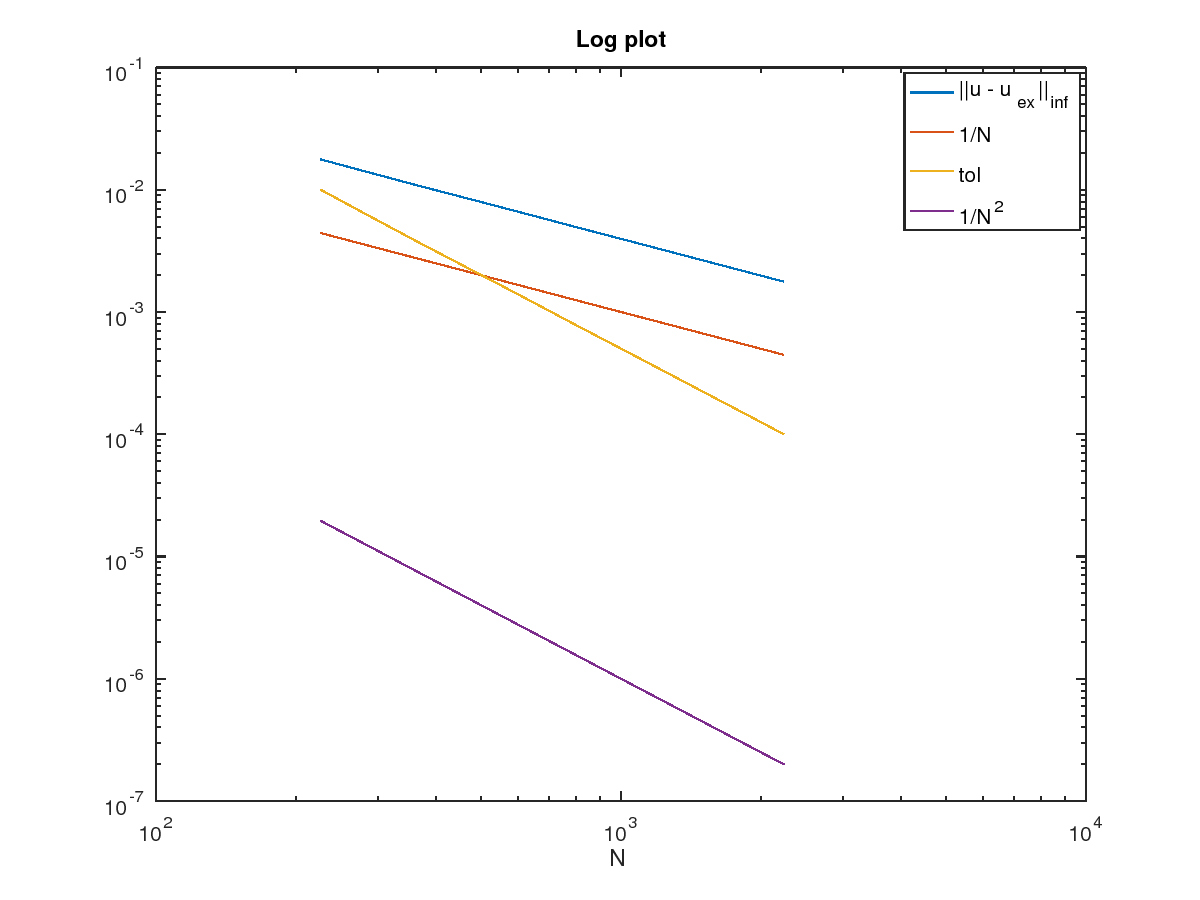
\includegraphics[width=1\linewidth]{time_order}
	\caption[Logarithmic plot of convergence orders is time adaptivity]{The logarithmic plot shows how tolerance , $ tol $, on the difference between the two approximations of the solution, that are numerical solution and initial guess, is of second order respect to $ \frac{1}{N} $, while the error, that is the norm of the difference between exact solution and numerical one, $|| u -u _{ex}||_{\infty}$, is of order one. That means that if an accuracy of $ 0.01 $ is required, then $tol$ has to be equal to $ 0.01^2 $ and, consequently, $ 100 $ time steps will be computed. }
	\label{time_order}
\end{figure}
\section{Space discretization}
The mesh that we decided to use has the quadtrees' numeration for the nodes (see \cite{p4est}). Before going in more details, we will discuss about some difficulties that we have encountered. \\
In view of the fact that we have to solve nonlinear systems, we used the C++ library LIS (Library of Iterative Solvers for linear systems), that, as the name suggests, solves liner problems with iterative methods. Since we needed to implement parallel solving to make the computing time reasonable, we created an interface for LIS, \texttt{lis\_distributed\_class}, in the library that we used for our implementations, called BIM, that manage a "decentralized" parallelization. This means that if we consider a linear system $ A u = f $, each processor will have  only his piece of $ A $, $ u $ and $ f $. In particular LIS requires matrix $ A $ to be divided in strictly separated ranges of rows. Also vectors $ u $ and $ f $ have to be divided among processors with the same ranges. The point is that the numeration that we have chosen for the mesh, does not divide matrix and vectors as LIS requires in a parallel environment. \\
Let see what happens and how we handled with it.
\subsection{Numeration of quadtrees meshes}
As we said above, solver LIS requires to have the matrix $ A $ divided by rows whenever it is asked parallel solving. For example, if we have a matrix with dimension $ 25 \times 25 $ and we want to parallelize it with 2 processors, then the first processor will have the first 15 rows, while the second one the others 10. \\
Let see how the numeration with quadtrees works for an uniform mesh. Just to fix the ideas, imagine to have a mesh of $ 4 \times 4 $ quadrants, that is $ 5 \times 5 $ nodes. The numeration starts form the first quadrant of the first row from the top down and it is done in this order: \\
\begin{center}
	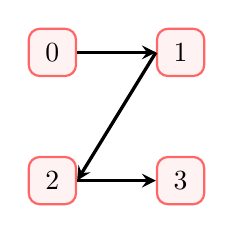
\begin{tikzpicture}[
	squarednode/.style={rectangle, draw=red!60, fill=red!5, thick, minimum size=6mm},
	]
	\centering
	
	%Nodes
	\node[squarednode]      (nodo1)                              {0};
	\node[squarednode]        (nodo2)       [right=of nodo1] {1};
	\node[squarednode]      (nodo3)       [below=of nodo1] {2};
	\node[squarednode]        (nodo4)       [right=of nodo3] {3};
	
	%Lines
	\draw[->] (nodo1.east) -- (nodo2.west);
	\draw[->] (nodo2.west) -- (nodo3.east);
	\draw[->] (nodo3.east) -- (nodo4.west);
	\end{tikzpicture}
\end{center}
Nodes in all quadrants are numerated with this order and also the sequence of quadrants that are taken has the same logic, as is shown in Figure \ref{mesh5x5}. With this procedure the final numeration of all the nodes of a $ 5 \times 5 $  mesh results to be the one in Figure \ref{nodimesh5x5}.
\begin{figure}[h]
	\centering
	\includegraphics[width=0.7\linewidth]{mesh5x5}
	\caption[Sequence of quadrants taken in quadtrees numetation for a mesh $ 5\times 5 $]{Sequence of quadrants taken to numerated}
	\label{mesh5x5}
\end{figure}

\begin{figure}[h]
	
	\centering
	\includegraphics[width=0.7\linewidth]{nodimesh5x5}
	\caption[Quadtrees numeration of nodes for a mesh $ 5 \times 5 $]{Quadtrees numeration of a $ 5 \times 5 $ mesh}
	\label{nodimesh5x5}
\end{figure}
With a mesh of this dimension, in discrete approximation all the space variables, will turn into  vectors of $ 5^2 = 25 $ components. Therefore the linear system that we have to solve has the shape $ A u = f $, with $ A \in \mathbb{R}^{25} \times \mathbb{R}^{25} $ and  $ u,f \in \mathbb{R}^{25} $. Since our system is coming from advection-diffusion-reaction equations, the most general pattern that matrix $ A $ can have is the one implemented by the method  called \texttt{bim2a\_structure (tmsh, A)} of class \texttt{sparse\_matrix}. This pattern is supposed to compare each node with all its four neighbours, because the problem has diffusion term and, indeed $ A $ has to contain also the discrete gradient of the variable $ u $. For example, in row 6, the previous method will allocate memory in $ A $, in column 6, 2, 7 and 15.\\
If we decide to solve the system with more processors, for example two, then the mesh in Figure \ref{nodimesh5x5} will be split in two parts. All the first 8 quadrants with their nodes will be of processor 1, and the other 8 will go to processor 2. Shared nodes, also called local nodes, that is nodes on the border of quadrants belonging to different processors, will be owned by the first processor that "touches" them. Therefore, in our example nodes 6, 7, 8, 13 and 14, will be owned by processor 1. But then, what happens to the matrix $ A $ ? Each processor will have only cells of the global matrix that link nodes owned by that processors or shared. In our case, processor 1 will have those cells of $ A $ that have indexes less or equal to the number of the last node owned by it, that is node 14. So, it will not have, for example, cells (14,22) or (6,15), that are actually present in rows 14 and 6 in the global matrix.
Figure \ref{patterndivision} shows how the patter of the global matrix is divided, in particular blu elements are of processor 1 while red of processor 2. As we can see there are overlaps that are all the red elements in the processor 1 's region. In fact, in those positions, both processors have their contribution, and to obtain the values of the global matrix, we have to sum them.\\
\begin{figure}[h]
	
	\centering
	\includegraphics[width=0.7\linewidth]{pattern_division}
	\caption[Patter of a matrix come from a mesh $ 5 \times 5 $ ]{It is illustrated the pattern of global matrix $ A $, blu cells are owned by processor 1 and red by processor 2. Where we see red elements in the region of processor 1, it means that there are overlaps, both processors has a value for that cells, and the sum of them gives the value of the global matrix. From this plot is clear that the division of a mesh with quadtrees numerations among processors is not made row by row, as LIS requires. }
	\label{patterndivision}
\end{figure}
The point of this introduction of quadtrees mesh, actually, is to show that the natural separation among processors of the mesh's regions, so of A, is not divided by rows, and there are even overlaps for same elements. Having said that, we already know that LIS wants matrix $ A $ to be strictly separated by rows, so our next aim was to create a new version of the already existing class in BIM of sparse matrices called \texttt{sparse\_matrix}, that handles this problem.
\subsection{Sparse matrix distributed class}
In this section, we present the alternative of class \texttt{sparse\_matrix}, that was created to allow each processor to assemble its matrix as LIS solver requires. This class is called \texttt{distributed\_sparse\_matrix} and its main variables are the following. 
\\
\\
\begin{lstlisting}[language=C++, caption={class distributed\_sparse\_matrix}]
class
distributed_sparse_matrix
: public sparse_matrix
{
private :
void
non_local_csr_index ();
void
non_local_csr_value ();
size_t is, ie;
MPI_Comm comm;
int mpirank, mpisize;
int nnz_owned;
struct
non_local_t
{
std::vector<int> prc_ptr, row_ind, col_ind;
std::vector<double> a;
} non_local;
std::map<int, std::vector<int>> row_buffers;
std::map<int, std::vector<int>> col_buffers;
std::map<int, std::vector<double>> val_buffers;
std::vector<int> ranges;
std::vector<int> rank_nnz;
public :
void
set_ranges (size_t is_, size_t ie_, MPI_Comm comm_ =     
MPI_COMM_WORLD);
distributed_sparse_matrix (size_t is_, size_t ie_,
MPI_Comm comm_= MPI_COMM_WORLD)
: mapped (false)
{ set_ranges (is_, ie_, comm_); }
distributed_sparse_matrix (MPI_Comm comm_ = MPI_COMM_WORLD)
: comm (comm_), mapped (false)
{ }
\end{lstlisting}

Let $ A $ be a matrix of type \texttt{distributed\_sparse\_matrix}. First of all, we have to set variables \texttt{is} and \texttt{ie}, which indicate the first and the last row owned by the current rank. These are computed in \texttt{lis\_distributed\_class} and passed to $ A $ by a method in the following way: \texttt{A.set\_ranges (is, ie)}. This sets also the components of \texttt{ranges}, that is the rows' ranges in which the global matrix is divided among the processors.\\
In lines 15-19 it is defined the structure \texttt{non\_local} that has \texttt{prc\_ptr}, a vector supposed to contain the numbers of nonzero elements that local A has in each range. Differently from vector \texttt{ranges}, \texttt{prc\_ptr}, like all the others, changes from rank to rank; indeed each rank has a different $ A $. So this is a way to indicate how many elements and to who the current rank has to communicate. The other vectors in \texttt{non\_local} are basically the indexes and values in AIJ format of the elements of A out of the range of current rank. All of them are computed by \texttt{non\_local\_csr\_index}. 
\begin{lstlisting}[language=C++, caption={distributed\_sparse\_matrix::non\_local\_csr\_index ()}]
void
distributed_sparse_matrix::non_local_csr_index ()
{
non_local.row_ind.clear ();
non_local.col_ind.clear ();
non_local.a.clear ();
this->set_properties ();
non_local.prc_ptr.assign (this->mpisize + 1, 0);
sparse_matrix::col_iterator jj;
for (size_t ii = 0; ii < this->mpisize; ++ii)
{
non_local.prc_ptr[ii+1] = non_local.prc_ptr[ii];
if (ii != mpirank)
for (size_t kk = ranges[ii]; kk < ranges[ii+1]; ++kk)
{
non_local.prc_ptr[ii+1] += (*this)[kk].size ();
non_local.col_ind.reserve ((*this)[kk].size ());
non_local.row_ind.reserve ((*this)[kk].size ());
for (jj  = (*this)[kk].begin ();
jj != (*this)[kk].end (); ++jj)
{
non_local.row_ind.push_back (kk);
non_local.col_ind.push_back 
(this->col_idx (jj));
non_local.a.push_back (this->col_val (jj));
}
}
}
non_local.a.resize (non_local.row_ind.size ());
}
\end{lstlisting}
As we see, \texttt{prc\_ptr} is, actually, the cumulative sum of the number of nonzero elements in the others ranges. We also see that with the check in line 13, only out-of-range elements are considered.\\
Up to now, for each $ A $ implemented by different ranks, we can identify which elements of the matrix are out of the current processor's range and to which range they below, therefore to which rank they have to be communicated. Going back to Figure \ref{patterndivision} and taking the ranges $ (0,14) $ for rank 0 and $ (15,25) $ for rank 1, matrix $ A $ of rank 0 will have empty vectors in \texttt{non\_local} structure, because its elements are all in the current range, while rank 1 will have \texttt{non\_local} vectors of size 18, since this is the number of its elements that stay in rank 0 's range. Now the aim is to communicated these components to rank 0.
\begin{lstlisting}[language=C++, caption={distributed\_sparse\_matrix::remap ()}]
void
distributed_sparse_matrix::remap ()
{
non_local_csr_index ();
/// Distribute buffer sizes
rank_nnz.assign (mpisize, 0);
for (int ii = 0; ii < mpisize; ++ii)
rank_nnz[ii] = non_local.prc_ptr[ii+1] 
- non_local.prc_ptr[ii];
MPI_Alltoall (MPI_IN_PLACE, 1, MPI_INT, &(rank_nnz[0]), 1,
MPI_INT, comm);
/// Allocate buffers
for (int ii = 0; ii < mpisize; ++ii)
if ((rank_nnz[ii] > 0) && (ii != mpirank))
{
row_buffers[ii].resize (rank_nnz[ii]);
col_buffers[ii].resize (rank_nnz[ii]);
val_buffers[ii].resize (rank_nnz[ii]);
}
/// Communicate overlap regions
/// 1) communicate row_ptr
std::vector<MPI_Request> reqs;
for (int ii = 0; ii < mpisize; ++ii)
{
if (ii == mpirank) continue; // No communication to self!
if (rank_nnz[ii] > 0) // we must receive 
//something from rank ii
{
int recv_tag = ii   + mpisize * mpirank;
reqs.resize (reqs.size () + 1);
MPI_Irecv (&(row_buffers[ii][0]), row_buffers[ii].size (),
MPI_INT, ii, recv_tag, comm, &(reqs.back ()));
}
int rank_nnz_snd_ii = non_local.prc_ptr[ii+1] -
non_local.prc_ptr[ii];
if (rank_nnz_snd_ii > 0) // we must send something to rank ii
{
int send_tag = mpirank + mpisize * ii;
reqs.resize (reqs.size () + 1);
MPI_Isend (&(non_local.row_ind[non_local.prc_ptr[ii]]),
rank_nnz_snd_ii, MPI_INT, ii, send_tag, comm,
&(reqs.back ()));
}     
}
MPI_Waitall (reqs.size (), &(reqs[0]), MPI_STATUSES_IGNORE);
reqs.clear ();
/// 2) communicate col_ind
for (int ii = 0; ii < mpisize; ++ii)
{
if (ii == mpirank) continue; // No communication to self!
if (rank_nnz[ii] > 0) // we must receive 
// something from rank ii
{
int recv_tag = ii   + mpisize * mpirank;
reqs.resize (reqs.size () + 1);
MPI_Irecv (&(col_buffers[ii][0]), col_buffers[ii].size (),
MPI_INT, ii, recv_tag, comm, &(reqs.back ()));
}
int rank_nnz_snd_ii = non_local.prc_ptr[ii+1] -
non_local.prc_ptr[ii];
if (rank_nnz_snd_ii > 0) // we must send 
// something to rank ii
{
int send_tag = mpirank + mpisize * ii;
reqs.resize (reqs.size () + 1);
MPI_Isend (&(non_local.col_ind[non_local.prc_ptr[ii]]),
rank_nnz_snd_ii, MPI_INT, ii, send_tag, comm,
&(reqs.back ()));
}     
}
MPI_Waitall (reqs.size (), &(reqs[0]), MPI_STATUSES_IGNORE);
reqs.clear ();
mapped = true;
update = true;
}
\end{lstlisting}
Here we encounter \texttt{row\_buffers}, \texttt{col\_buffers} and \texttt{val\_buffers} that basically are containers of the elements that the current rank receives from the others. The numbers of these elements are set in the vector \texttt{rank\_nnz} with \texttt{MPI\_Alltoall} (lines 7-12). With this numbers, we set buffers' sizes . \\
Now comes the crucial part, in which each rank sends the indexes of its non local elements and receives the others' non local elements that are in its range. With line 25, communication to itself is avoided and the procedure of sending and receiving is done only if actually there is some thing to send or receive. Therefore, essentially, \texttt{distributed\_sparse\_matrix::remap ()} set the indexes of the cells in $ A $ in which each processor has to receive a value. For the communication of these values, we made the next method.
\begin{lstlisting}[language=C++, caption={distributed\_sparse\_matrix::assemble ()}]
void
distributed_sparse_matrix::assemble ()
{
if (! mapped)
remap ();
non_local_csr_value ();
/// 3) communicate values
std::vector<MPI_Request> reqs;
for (int ii = 0; ii < mpisize; ++ii)
{
if (ii == mpirank) continue; // No communication to self!
if (rank_nnz[ii] > 0) // we must receive something 
// from rank ii
{
int recv_tag = ii   + mpisize * mpirank;
reqs.resize (reqs.size () + 1);
MPI_Irecv (&(val_buffers[ii][0]), val_buffers[ii].size (),
MPI_DOUBLE, ii, recv_tag, comm, &(reqs.back
()));
}
int rank_nnz_snd_ii = non_local.prc_ptr[ii+1] -
non_local.prc_ptr[ii];      
if (rank_nnz_snd_ii > 0) // we must send something 
// to rank ii
{
int send_tag = mpirank + mpisize * ii;
reqs.resize (reqs.size () + 1);
MPI_Isend (&(non_local.a[non_local.prc_ptr[ii]]),
rank_nnz_snd_ii, MPI_DOUBLE, ii, send_tag,
comm, &(reqs.back ()));
}     
}
MPI_Waitall (reqs.size (), &(reqs[0]), MPI_STATUSES_IGNORE);
reqs.clear ();
/// 4) insert communicated values into sparse_matrix
for (int ii = 0; ii < mpisize; ++ii) // loop over ranks
if (ii != mpirank)
for (int kk = 0; kk < rank_nnz[ii]; ++kk)  
(*this)[row_buffers[ii][kk]][col_buffers[ii][kk]]
+= val_buffers[ii][kk];
/// 5) zero out communicated values  
for (int iprc = 0; iprc < mpisize; ++iprc)
if (iprc != mpirank)
{
for (int ii = non_local.prc_ptr[iprc];
ii < non_local.prc_ptr[iprc+1]; ++ii)
// the following will throw if we try to access
// an element which does not exist yet!
(*this)[non_local.row_ind[ii]].at (non_local.col_ind[ii])
= 0.0;
}
if (update)
{
nnz_owned = 0;
for (int irow = is; irow < ie; ++irow)
nnz_owned += (*this)[irow].size ();
}
update = false;
}
\end{lstlisting}
In nonlinear solving of partial differential equations problems, often, pattern of the matrix $ A $ remains the same for all the nonlinear and, eventually, time steps. This is why we actually separated the communications of the indexes from the one of the values; indeed, ones computed, \texttt{row\_buffers} and \texttt{col\_buffers} are supposed to remain the same, therefore there is no need to calculate them every time. Actually, the same is true also for the \texttt{non\_local} structure of $ A $. This is why we implemented also the method \texttt{non\_local\_csr\_value ()}, that updates only the values of \texttt{non\_local.a}. Regarding the buffers, communication of the values is essentially the same as before and, it is in lines 36-40, that the communicated values are inserted in matrix $ A $. At the end all the out-of-range values of $ A $ are set to zero.\\
\subsection{Distributed vector class}
In our example of linear system $ Au = f $, we know that every rank has his own matrix $ A $ and that the sum of all of them represents the global matrix. Since $ (A_1 + A_2) (u_1 + u_2) \neq A_1 u_1 + A_2 u_2$, $ u $ has to have the global values, but it is enough to allocate the ones that correspond to owned and shared nodes, and not to all the nodes, since $ A $ has nonzero elements only for these nodes. On the other hand, $ f $ could have elements different from zero only where $ A $ has nonzero rows, that is in all owned and shared nodes. But, again, if we want to pass this vectors in LIS for parallel solving, we have to pass just the piece of the current range, and it means that all the out-of-range values has to bo communicated to their correspondent processors.
For this regard, we implemented a new class called \texttt{distributed\_vector}. Let see how is structured.
\begin{lstlisting}[language=C++, caption={distributed\_vector class}]
class
distributed_vector
{
private:
MPI_Comm comm;
int mpirank;
int mpisize;
bool mapped;
int owned_count;
int is, ie;
/// vector entries owned by the current node
std::vector<double> owned_data;
/// vector entries touched by the current node
/// that belong somwhere else
std::map<int, double> non_local_data;
/// Structure to hold data of ghost entries
/// in a format amenable for send/receive
struct
ghosts_t
{
std::vector<int> prc_ptr, row_ind, rank_nnz;
std::vector<double> a;
} ghosts;
/// Copy data from non_local_data to ghosts
void
ghost_csr ();
/// Update ghosts.
void
ghost_csr_update ();
/// Structure to hold data of ghost entries
/// in a format amenable for send/receive
struct
mirrors_t
{
std::vector<int> prc_ptr, row_ind, rank_nnz;
std::vector<double> a;
} mirrors;
/// the entries that are owned by rank i
/// are numbered between ranges[i]
/// and ranges[i+1]
std::vector<int> ranges;
/// check whether the idx-th global
/// entry is owned by the current rank
inline bool
is_owned (int idx) const
{ return idx >= is && idx < ie; }
/// check whether the idx-th global
/// entry is owned by the given rank
inline bool
is_owned (int idx, int irank) const
{ return idx >= ranges[irank] && idx < ranges[irank+1]; }
/// return the rank that owns the idx-th entry
inline int
owner (int idx)
{
auto ir = std::lower_bound (ranges.begin (), 
ranges.end (), idx);
return int ((ir - ranges.begin ()) - 1);
}
public:
distributed_vector (int owned_count_,
MPI_Comm comm_ = MPI_COMM_WORLD);
distributed_vector (int is_, int ie_,
MPI_Comm comm_ = MPI_COMM_WORLD);
distributed_vector () {};
void
set_owned_count (int owned_count_, MPI_Comm comm_ =  
MPI_COMM_WORLD);
\end{lstlisting}
First of all, let have a look at the constructors. Suppose to have a distributed vector $ u $, when we declare it, we have also to provide either the dimension or the extremes of the owned nodes' range. If it is not possible, because, for example we are declaring this kind of vectors in a class that does not have this information internally, then we can declared it without anything, but when we want to use really that vector, we must implement first \texttt{u.set\_owned\_count (dimension\_range)}. This is because the first two constructors and that method set the size of \texttt{owned\_data}, which with \texttt{non\_local\_data}, is the main container of the class. Indeed, the first one is meant to contain values of the owned nodes, so the values that ere in the range of the current rank. The second will contain eventually the values and their indexes of out-of-range elements. Structures \texttt{ghosts} and \texttt{mirrors} has the same role as \texttt{non\_local} and \texttt{buffers} in \texttt{distributed\_sparse\_matrix}. The first one, that contains the non local elements, is computed  with private method \texttt{ghosts\_csr ()}, while the second one is computed after the communications done in methods called \texttt{remap ()} and \texttt{assemble ()}, analogue at the ones of the matrix's class, and contains the elements that are in the current range and are sent from the other ranks. All the mechanism of sending and receiving is very similar to the one shown in the previous section, so we will limit ourselves to recall the main steps. 
\begin{enumerate}
	\item  copy \texttt{non\_local\_data} into ghosts structure;
	\item  send ghosts indexes and receive into mirrors;
	\item add mirrors into \texttt{owned\_data};
	\item copy \texttt{owned\_data} into mirrors;
	\item send mirrors data and receive into ghosts;
	\item copy ghosts data into non\_local\_data.
\end{enumerate}
The two first steps are of the method \texttt{remap ()}, while the others are in \texttt{assemble ()}. Besides, steps 4, 5 and 6 were not present in the previous class. They are a kind of inverse communication, indeed after the update of \texttt{owned\_data}, this one is communicated to the others' \texttt{non\_local\_data}. In this way, we ensure that also \texttt{non\_local\_data} will be updated with the global values. This needs to happen because, as we said before, $ u $ has to have the global values also out-of-the range.\\
The use of objects of this class is quite easy since is sufficient to write \texttt{u[i] = val} and, if  \texttt{i} belong to the current range, then it is equivalent to write \texttt{owned\_data[i] = val}, otherwise it is inserted a new component \texttt{<i, val>} in the map \texttt{non\_local\_data}, or it is updated, if one exists already with this index. It is enough to initialize all the elements out-of-range that we are interested to keep inside $ u $, and then they will be always updated with \texttt{assemble ()}. In our case, they will be the shared nodes.\\

\chapter{Newton methods for nonlinear problems}
Often in mathematical modeling nonlinear equations can be encountered and it is quite common that they can not be solved analytically. In this case, therefore, the solutions must be approached using \textit{iterative methods}.
In this chapter we will address the main aspects of theory of the Newton's method, which is a particular case of \textit{fixed point iteration method}. This will be useful to prepare the ground for the numerical method that we have planned to test. \\
First of all we will introduce the standard Newton's method for nonlinear problems, in which each step solves a linear system where left-hand-side is the Jacobian of the nonlinear system and right-had-side the evaluation of the problem in a guess, that is computed from the previous step. Only the fist guess is chosen, and we will see the importance of this choice, since the convergence is local. Then we will list some of the most common \textit{quasi Newton's methods}, that are methods in which the Jacobian is approximated, and indicate how the convergence is affected. On the other hand, also \textit{quasi-Newton methods} will be introduced, that, at each step, solve the linear system non exactly. Our concern will be on Newton-Krylov methods and, in particular, on the Generalized Minimal Residual (GMRES). In section 3.2 we will give an idea of why quasi-Newton methods and inexact Newton methods can be seen as equivalent. \\
In the end, we will illustrate some common techniques meant to globalizate the convergence, with more focus on line search approach. 
 
\section{Introduction of the Method}
Let us consider this nonlinear problem 
\begin{equation*}
\begin{cases}
F(\textbf{x}) = 0\\\textbf{x} \in \mathbb{R}^n,
\end{cases}
\end{equation*}
where $F: \mathbb{R}^{n} \rightarrow \mathbb{R}^{n}$ is continuously differentiable.\\
Newton's method is an iterative method and its sequence is
\begin{equation}
{\textbf{x}}_{k+1} = {\textbf{x}}_{k} - F'({\textbf{x}}_{k})^{-1} F({\textbf{x}}_{k}), 
\label{Newton_it}
\end{equation}
where we start from a initial guess ${x}_{0}$. We can view \eqref{Newton_it} as the two-term Taylor expansion in which we impose $F({\textbf{x}}_{k+1})=0$.  Therefore, at each step $ \textbf{x}_{k+1} $ is an approximation of the solution.\\

We introduce some assumptions and definitions useful for the convergence's theory.\\
\textbf{Standard assumptions:} 
\begin{itemize}
	\item $F(\textbf{x}) = 0$ has a solution ${x}^{*}$;
	\item $F'(\textbf{x}): \Omega \rightarrow \mathbb{R}^{n}$ is Lipschitz continuous;
	\item $F'({\textbf{x}}^{*})$ is non singular.
\end{itemize}
\noindent \textbf{Convergence's definitions}: \textit{ Let $\alpha \in \mathbb{R}^{n}$ and ${\textbf{x}}_{k} \in \mathbb{R}^{n}$, $k = 0,1,2,...$ Then ${\textbf{x}}_{k}$ is said:}
	
	\begin{itemize}
		\item \textit{ \textbf{q-linearly convergent} if there exists a constant $C \in (0,1)$ and an integer $m$ such that for all $k\geq m$ 
		\begin{equation*}
		||{\textbf{x}}_{k+1}-\alpha|| \leq C||{\textbf{x}}_{k}-\alpha|| .
		\end{equation*}	}
	    \item \textit{ \textbf{q-superlinearly convergent} if there exists a sequence ${{C}_{k}}$ convergent to 0 such that
		\begin{equation*}
		||{\textbf{x}}_{k+1}-\alpha|| \leq C_k||{\textbf{x}}_{k}-\alpha|| .
		\end{equation*}}
	
	\item \textit{ \textbf{convergent sequence of q-order p} $(p > 1)$ if there exists a
		constant $C$ and an integer $m > 0$ such that for all $k \geq m$
		\begin{equation*}
		||{\textbf{x}}_{k+1}-\alpha|| \leq C{||{\textbf{x}}_{k}-\alpha||}^{p} .
		\end{equation*}}
\end{itemize}

\begin{theorem}
	\label{converg}
 Let the standard assumptions hold. Then there is a $\delta > 0$ such that, if the initial guess ${\textbf{x}}_{0} \in \mathit{B(\delta)}$, then the Newton iteration \eqref{Newton_it} converges q-quadratically to ${\textbf{x}}^{*}$, that is $||{\textbf{e}}_{k+ 1}|| \leq C ||{\textbf{e}}_{k}||$, for some $ C > 0 $ and with $ ||{\textbf{e}}_{k}|| = ||{\textbf{x}}_{k} - \textbf{x}_{ex}|| $ .
\end{theorem}
Since the initial guess needs to be "sufficiently near" to the solution, the convergence of the Newton's method is local.\\

A practical problem is that, in general, we do not have the analytical solution $\textbf{x}_{ex}$, so we can not calculate the error $||{\textbf{e}}_{k}|| = ||{\textbf{x}}_{k} - \textbf{x}_{ex}|| $. Therefore, we have to find another estimation of the error that can be used as an \textit{arrest criterion} of the iterate method.
For example, it is used the \textit{relative nonlinear residual} $||F(\textbf{x})||/||F({\textbf{x}}_{0})||$, that is a good indicator of size of the error, but only when $F'({\textbf{x}}^{*})$ is well conditioned. Indeed we have:
\begin{lem}
 Let the standard assumptions hold and $\delta > 0$ be small enough. Then for all $\textbf{x} \in \mathit{B(\delta)}$
\end{lem}

\begin{equation*}
\frac{||\textbf{e}||}{4 ||{\textbf{e}}_{0}|| \mathit{k}(F'({\textbf{x}}^{*}))} \leq \frac{||F(\textbf{x})||}{||F({\textbf{x}}_{0})|} \leq \frac{4 \mathit{k}(F'({\textbf{x}}^{*}))||\textbf{e}||}{||{\textbf{e}}_{0}||}
\end{equation*}
\textit{where $\mathit{k}(F'({\textbf{x}}^{*})) =||F'({\textbf{x}}^{*})||$ $ ||{F'({\textbf{x}}^{*})}^{-1}|| $ is the condition number of $F'({\textbf{x}}^{*})$ relative to the norm $||\cdot||$.}

\noindent Another way to decide whether to terminate is to look at the Newton \textit{step}
\begin{equation*}
{\textbf{s}}_{k+1} ={\textbf{x}}_{k+1} - {\textbf{x}}_{k}= -{F'({\textbf{x}}_{k})}^{-1}F({\textbf{x}}_{k}),
\end{equation*}
and except $ \textbf{x}_{k+1} $ as good approximation of the solution when $||{\textbf{s}}_{k+1}||$ is sufficiently small. This criterion is based on Theorem \ref{converg} which implies that 
\begin{equation*}
||{\textbf{e}}_{k+1}|| = ||{\textbf{s}}_{k+1}|| + \mathcal{O}({||{\textbf{e}}_{k+1}||}^{2}).
\end{equation*}
Hence, near the solution $\textbf{s}$ and $\textbf{e}$ are essentially the same size.\\ 

Sometimes it is too expensive from a computational point of view to evaluate $F'(\textbf{x})$ at each step and sometimes, actually, there is no need to be so precise because, for example, we are too far from the solution. And also we would like to have a global convergence, instead just of a local one. There are many techniques that are done for these requirements, and in the next session we illustrate some of them.
\section{Review of Variants of the Newton Method}
This section will regard mainly different ways to approximate ${F'}^{-1}$, but first of all we want to give a theoretical result about inaccuracy. Suppose that $F + \epsilon$ and $F' + \Delta$ are used instead of $F$ and $F'$ in the iteration, then we have the following result.
\begin{theorem}
	\label{accuracy}
	Let the standard assumptions hold. Then there are $K>0$, $\delta>0$ and $\delta_1>0$ such that if $\textbf{x}_{k} \in \mathit{B}(\delta)$ and $||\Delta(\textbf{x}_{k}) ||<\delta_1$ then 
 \begin{equation*}
 \textbf{x}_{k+1}=\textbf{x}_{k} - (F'(\textbf{x}_k)+\Delta(\textbf{x}_k))^{-1}(F(\textbf{x}_k)+\epsilon(\textbf{x}_k))
 \end{equation*}
	is defined (i.e.,$F'(\textbf{x}_k)+\Delta(\textbf{x}_k)$ is nonsingular) and satisfies 
\begin{equation*}
||{\textbf{e}}_{k+1}|| =K(||{\textbf{e}}_{k}||^2 + ||\Delta(\textbf{x}_n)|||\textbf{e}_k ||+||\epsilon(\textbf{x}_k) || ).
\end{equation*}
	
\end{theorem} 
As we observe, it can happen that the convergence is not quadratical anymore. 
\subsection{Quasi-Newton methods} 
Under this name we have all the Newton methods that do not calculate the real value of ${F'(\textbf{x})}^{-1}$, but use approximations. The price for such an approximation is that the nonlinear iteration converges more slowly; i.e., more nonlinear iterations are needed to solve the problem. However, the overall cost of solving is usually smaller, because the computation of the Newton step is less expensive.
Therefore, we are obligated to use a quasi-Newton method when is unavailable to have the exact expression of ${F'(\textbf{x})}^{-1}$ or is too expensive to compute it at every iteration. \\
Let us illustrate same of this methods. \\

\subsubsection{Chord method or modified Newton method} In this case the Newton iteration is given by
\begin{equation*}
{\textbf{x}}_{k+1} = {\textbf{x}}_{k} - F'({\textbf{x}}_{0})^{-1} F({\textbf{x}}_{k}) .
\end{equation*}
Suppose again that the standard assumptions hold. Assuming that the initial iteration is near enough to the solution ${\textbf{x}}^{*}$, the convergence of the chord iteration is q-linear. Indeed, this comes from Theorem \ref{accuracy}, noticing that $\epsilon(\textbf{x}_k) = 0$ and $||\Delta(\textbf{x}_k)|| = \mathcal{O}(||\textbf{e}_0||)$.\\
 In general, we can also update $F'(\textbf{x})^{-1}$ after $m$ iterations and not use $F'({\textbf{x}}_{0})^{-1}$ always.\\
A general way to implement chord-type methods is 
\begin{equation*}
{\textbf{x}}_{k+1} = {\textbf{x}}_{k} - {A}^{-1} F({\textbf{x}}_{k}), 
\end{equation*}
where $A \approx F'({\textbf{x}}^{*})$. Also in this case, if we have a good guess ${\textbf{x}}_{0}$ and $A$ is a good approximation of $ F'({\textbf{x}}^{*})$, then we have a \textit{q-linear} convergence. \\

\subsubsection{Shamanskii method} It consists in a alternation of a Newton step with a sequence of chord steps and leads to a class of \textit{high-order methods}, that is, methods that converge q-superlinearly with q-order larger that 2. \\
We can describe the transition from ${\textbf{x}}_{k}$ to ${\textbf{x}}_{k+1}$ by
\begin{gather*}
{\textbf{y}}_{1} = {\textbf{x}}_{k} -{F'({\textbf{x}}_{k})}^{-1}F({\textbf{x}}_{k}),\\
{\textbf{\textbf{y}}}_{j+1} = {\textbf{y}}_{j} -{F'({\textbf{x}}_{k})}^{-1}F({\textbf{y}}_{j}) \; \; \; \; \; for\; 1\leq j \leq m-1, \\
{\textbf{x}}_{k+1} = {\textbf{y}}_{m}
\end{gather*}

Note that for $m=1$ it is Newton's method and for $m=\infty$ it is the simplest chord method.
\begin{theorem}
	Let the standard assumptions hold and let $m \geq 1$ be given. Then there are $K_{S}>0$ and $\delta>0$ such that if $\textbf{x}_{0} \in \mathit{B(\delta)}$, the Shamankii iterates converge q-superlinearly to $\textbf{x}^{*}$ with q-order $m+1$ and 
	\begin{equation*}
	||\textbf{e}_{k+1} ||\leq K_{S} ||\textbf{e}_{k} ||^{m+1}.
	\end{equation*}
\end{theorem}
The advantage of the Shamanskii method over Newton's method is that hight q-order can be optained with far fewer Jacobian evaluations or factorizations.\\

\subsubsection{Difference approximations of the Jacobian matrix} Another possibility consists of replacing $F'(\textbf{x}_{k})$ with an approximation through \textit{n}-dimensional
differences of the form
\begin{equation*}
(F'^{k}_{h})_{j} = \frac{F(\textbf{x}_{k} + h^{k}_{j} \textbf{e}_{j}) - F(\textbf{x}_{k})}{h_{j}^{k}},\;\;  \forall k \geq 0,
\end{equation*}
	
where $\textbf{e}_j$ is the j-th vector of the canonical basis of $\mathbb{R}^n$ and $h_j^k>0$ are
increments to be suitably chosen at each step $k$ of the iteration.\\
 \textit{Convergence's result}. Under the standards assumptions, a initial guess "sufficiently near" to the solution and bounded $ h^{k}_{j}$ for $j=1,...,n$, then the sequence 
 \begin{equation}
   \textbf{x}_{k+1}=\textbf{x}_k -[F'^{k}_{h}]^{-1} F(\textbf{x}_k)
   \label{iter_conv_result}
 \end{equation}
 converges \textit{linearly} to $\textbf{x}^*$. Moreover, if there exists a
 positive constant $C$ such that $\max_{j}|h^{k}_{j}| \leq C ||\textbf{x}_k - \textbf{x}^*||$	or, equivalently,
 there exists a positive constant $c$ such that $\max_{j}|h^{k}_{j}| \leq c ||F(\textbf{x}_k)||$, then
 the sequence \eqref{iter_conv_result}, is convergent \textit{quadratically}. But we should pay attention also not to choose $h_j^k$ too small in order to avoid big errors of truncation. 
 \\
 
\subsubsection{Secant method}This case is done for single equations $f'(x) = 0$ and the derivative is approximated using a finite difference with the most recent two iterations. 
\begin{equation}
{x}_{k+1} = {x}_{k} -\frac{({x}_{k}-{x}_{k-1}) f({x}_{k})}{f({x}_{k})-f({x}_{k-1})} 
\label{it_secant_method}
\end{equation} 
For the computation of ${x}_{1}$, one option is to set ${x}_{-1} = 0.99{x}_{0}$. If the standard assumptions hold and $ x_{-1} $ and $ x_0  $ are sufficiently near the solution, Theorem \ref{accuracy}, with $\epsilon = 0$ and $||\Delta(x_k)||=\mathcal{O}(||e_{k-1}||)$, implies that the iteration converges\textit{ q-superlinearly}.\\
 \subsubsection{Broyden's method}This is a version of secant method for higher dimensions than 1.\\
In a multidimentional case the equation \eqref{it_secant_method} has no sense, because we can not divide by a vector, so we ask that ${B}_{k}$, the current approximation od $F'(\textbf{x})$, satisfies the secant equations 
\begin{equation*}
{B}_{k}({\textbf{x}}_{k} - {\textbf{x}}_{k-1}) = F({\textbf{x}}_{k}) - F({\textbf{x}}_{k-1}).  
\end{equation*} 
A wide variety of methods, that satisfy the secant equations, have been designed to preserve such properties of the Jacobian as the sparsity patter or symmetry. In the case of Broyden's method, we have
\begin{equation*}
{\textbf{x}}_{k+1} = {\textbf{x}}_{k} - {\lambda}_{k}{B}_{k}^{-1}F({\textbf{x}}_{k}).  
\end{equation*} 
where ${\lambda}_{k}$ is the step length for Broyden direction
\begin{equation*}
{\textbf{d}}_{k} = -{B}_{k}^{-1}F({\textbf{x}}_{k})  
\end{equation*} 
After the computation of ${\textbf{x}}_{k+1}$, ${B}_{k}$ is updated 
\begin{equation*}
{B}_{k+1} = {B}_{k} + \frac{(\textbf{y} - {B}_{k}\textbf{s}){\textbf{s}}^{T}}{{\textbf{s}}^{T}\textbf{s}}  
\end{equation*} 
with $\textbf{y} = F({\textbf{x}}_{k+1}) - F({\textbf{x}}_{k})$ and $ \textbf{s} = {\textbf{x}}_{k+1}-{\textbf{x}}_{k} = {\lambda}_{k}{\textbf{d}}_{k} $.\\
Broyden's method does not guarantee that the approximate Newton direction will be a descent direction for $||F||$  (the same can happen also with the secant method).
Under hypothesis of standard assumptions and both ${\textbf{x}}_{0}$ and ${B}_{0}$ are enough good approximations of $ \textbf{x}^* $ and $ F'(\textbf{x}^*) $, the convergence theory for Broyden's method is \textit{q-superlinear}. So it is only local and, therefore, less satisfactory than that for the Newton and Newton-Krylov methods (we will see in the next subsections). Moreover the line search cannot be proved to compensate for poor initial iterate, because it can work for sure only with a good approximation of $F'({\textbf{x}}_{k})$.
\\
 \subsubsection{Approximation of a sparse Jacobian}
 In general the advantages of approximating $ J_k $, the Jacobian matrix, instead of its inverse $ J_k^{-1} $, are more evident when we have a sparse Jacobian with known nonzero positions. Indeed the inverse matrix could not be sparse and so it could need a storage much bigger and, if we know the pattern of the matrix, we can directly set these values to zero and have less conditions to solve. By the way, this scenario is typical for differential nonlinear problems, for which the Jacobian is sparse with known pattern. \\
  We recall the general nonlinear problem $ F(\textbf{x}) = 0 $ and its iterative step:
 \begin{eqnarray*}
 J_k \textbf{s}_k = - F_k, \\
\textbf{x}_{k+1} = \textbf{x}_k + \lambda_k \textbf{s}_k,
 \end{eqnarray*}
 with $ \lambda_k $ a positive scalar, that reduces the length of the step to achieve stability, and $ J_k  $ approximation of the Jacobian matrix. 
 In order to find $ J_k $, we use first primary conditions, that impose to $ J_k $ to predict the same changes along the direction $ \textbf{s}_k $ as $ F_k $ does, therefore 
 \begin{equation}
 \label{prim}
 J_{k+1} = J_k + \frac{ [ F_{k+1} - (1-t_k) F_k ] \textbf{s}_k^T}{t_k \textbf{s}_k^T \textbf{s}_k}.
 \end{equation}
 So we need to find conditions for the $ n^2 -n $ unknowns that remain. These are called secondary conditions and they can be chosen differently, for example, $ J_k $ can be forced to give the same variations that $ F_k $ has along all orthogonal directions on $ \textbf{s}_k $.\\
  As we can see, the logic is the one used Broyden's method, but, here, it has to be adapted to the sparse case, below we see how.\\
  The $ i $th row $ g_k^{(i)} $ of $ J_k $ is an approximation to the gradient of the $ i $th function component $ F_k^{(i)} $. If $ n-r_i $ components of $g_k^{(i)} $ are known constants, we impose first the condition that these components shall remain unchanged in the Jacobian revision, and then we implement the other conditions on the basis of the remaining $ r_i $ coordinate directions.
  The vectors $ \hat{\textbf{s}}_k $ and $ \bar{g}^{(i)} $ are introduced, where the first one is a column vector that is the same as $ \textbf{s}_k $, but setting  $\textbf{s}_k^{(j)} $ to zero whenever the corresponding element of $ g_k^{(i)} $ is a known constant. Indeed, $ \bar{g}^{(i)} $ is a row vector that is as $ g_k^{(i)} $, but setting its unknown elements to zero. 
  The primary conditions becomes
\begin{equation}
\label{firstcond}
	t_k g_{k+1}^{(i)} \hat{\textbf{s}}_k = F_{k+1}^{(i)} -F_{k}^{(i)} - t_k \bar{g}^{(i)} \textbf{s}_k, \; \; \; i = 1,2,\dots,n.
\end{equation}
  This is identical to the primary condition $ t_k J_{k+1} \textbf{s}_k = F_{k+1} - F_k$, because $ g_{k+1}^{(i)} \hat{\textbf{s}}_k + \bar{g}^{(i)} \textbf{s}_k = g_{k+1}^{(i)} \textbf{s}_k$. \\
  The secondary condition is obtained in a similar way by restricting the previous secondary condition to the $ r_i $-space corresponding to the unknown elements of $ g_i $, that is:
  \begin{equation}
  \label{seccond}
  g_{k+1}^{(i)} \hat{q} = g_k^{(i)} \hat{q}, \; \; \; i = 1, 2, \dots, n,
  \end{equation}
  where $ \hat{q} $ satisfies $ \hat{\textbf{s}}_{k}^{T} \hat{q} = 0 $.
  It can be verified that \eqref{firstcond} and \eqref{seccond} are satisfied by the exact row-by-row analogue of \eqref{prim}, that is 
  \begin{equation*}
  g_{k+1}^{(i)} = g_{k}^{(i)} + \frac{ [ F_{k+1}^{(i)} - (1-t_k) F_k^{(i)} ] \hat{\textbf{s}}_k^T}{t_k \hat{\textbf{s}}_k^T \hat{\textbf{s}}_k}.
  \end{equation*}
  All this method is stated in \cite{Schubert} by L.K. Schubert and it is also shown that, when the dimension $ n $ increases, this approach is much better than classical Broyden's method for a sparse Jacobian.
  
\section{Inexact Newton Method} \label{inexact_Newton_method} Rather than approximate the Jacobian, one could instead solve the equation for the Newton step approximately. An inexact Newton method uses as a step a vector $\textbf{s}$ that satisfies the inexact Newton condition
\begin{equation}
||F'(\textbf{x}_k)\textbf{s}+F(\textbf{x}_k)|| \leq \eta ||F(\textbf{x}_k)||.
\label{inexact_newton}
\end{equation}
The parameter $\eta$ is called \textbf{forcing term}. Away from the solution $\textbf{x}^*$, $F$ and its local linear model may disagree considerably at a step that closely approximates the Newton step. So choosing $\eta$ too small may lead to \textit{oversolving} the Newton equation. Therefore far from the solution, a less accurate approximation of the Newton step may be both cheaper and more effective. So, the idea is to choose a forcing term that becomes smaller when the iteration are closer to the solution. And what about the convergence?
\begin{theorem} \label{convergenza_IN}
	Let the standard assumptions hold. Then there are $\delta$ and $\bar{\eta}$ such that, if $\textbf{x}_0 \in \mathit{B}(\delta)$, ${\eta_n}\subset [0,\bar{\eta}]$, then the inexact Newton iteration
	\begin{equation*}
	\textbf{x}_{k+1} = \textbf{x}_k + \textbf{s}_k
	\end{equation*}
	where
   \begin{equation*}
   ||F'(\textbf{x}_k)\textbf{s}_k+F(\textbf{x}_k)|| \leq \eta_k ||F(\textbf{x}_k)||,
   \end{equation*}
	converges q-linearly to $\textbf{x}^*$. Moreover, 
	\begin{itemize}
		\item if $\eta_n \rightarrow 0$, the convergence is q-superlinear, and 
		\item if $\eta_k \leq K_{\eta} ||F(\textbf{x}_k) ||^p$ for some $K_{\eta}>0$, the convergence is q-superlinear with q-order $1+p$.
	\end{itemize}
	
\end{theorem}
In literature, in particular \cite{Forcingterm}, we can find the following choices of $\eta$. \\
\noindent \textbf{Choice 1.} Given $\eta_0 \in [0,1)$, choose
\begin{equation}
\eta_k=\frac{||F(\textbf{x}_k) - F(\textbf{x}_{k-1}) - F'(\textbf{x}_{k-1})\textbf{s}_{k-1} ||}{||F(\textbf{x}_{k-1})||},\;\;\;\;\; k=1,2,3...
\label{Choice1.1}
\end{equation}
or
\begin{equation}
\eta_k=\frac{| ||F(\textbf{x}_k)|| - ||F(\textbf{x}_{k-1}) + F'(\textbf{x}_{k-1})\textbf{s}_{k-1} |||}{||F(\textbf{x}_{k-1})|| |},\;\;\;\;\; k=1,2,3...
\label{Choice1.2}
\end{equation}

 Note that $\eta_k$ given by \eqref{Choice1.1} and \eqref{Choice1.2} directly reflects the agreement between $F$ and its local linear model at the previous step. The choice \eqref{Choice1.2} may be more convenient to evaluate that \eqref{Choice1.1} in some circumstances. Since it is at least as small as \eqref{Choice1.1}, local convergence will be at least as fast as with \eqref{Choice1.1}.\\
 One possible way to obtain faster local convergence, while retaining the potential advantages of \eqref{Choice1.1} and \eqref{Choice1.2}, is to raise those expression to powers greater than one. \\
\noindent \textbf{Choice 2.} Given $\gamma \in [0,1]$, $\alpha \in (1,2]$, and $\eta_0 \in [0,1)$, choose
\begin{equation}
\eta_k=\gamma \left(\frac{||F(\textbf{x}_k)||}{||F(\textbf{x}_{k-1})||}\right)^{\alpha},\;\;\;\; k=1,2,3...
\label{Choice2}
\end{equation}
This choice does not directly reflect the agreement between $F$ and his local linear model. However, it can produce a little oversolving in practice.\\ 

In experiments it was observed that the forcing term choices occasionally become too small far away from a solution. There is a particular danger of the Choice 1 forcing terms becoming too small; indeed, a $\eta_k$ given by \eqref{Choice1.1} or \eqref{Choice1.2} can be undesirably small because of their very small step or coincidental very good agreement between F and its local linear model. For this reason there are \textbf{safegurads} that are intended to prevent the forcing term to become too small too soon.\\
\textit{Choice 1 safeguard}: Modify $\eta_k$ by $\eta_k = max  \{\eta_k, \eta_{k-1}^{\frac{(1+\sqrt{5})}{2}}\}$ whenever $\eta_{k-1}^\frac{(1+\sqrt{5})}{2} > 0.1$.\\
\textit{Choice 2 safeguard}: Modify $\eta_k$ by $\eta_k = max  \{\eta_k,\gamma  \eta_{k-1}^\alpha\}$ 
whenever $\gamma  \eta_{k-1}^\alpha > 0.1$.\\
As we can see, they are activated when the previous $ \eta $ was not so small as the new one tries to be, so it is more suspicious. \\
There is also another version of safeguard for the choice 2 in \cite{Kelley1}, and this is 
\begin{equation*}
\eta_k = min (\eta_{max}, max (\eta_k^C, 0.5 \tau_t/||F(\textbf{x}_k)||)),
\end{equation*}
with $\tau_t =  \tau_a + \tau_r||F(\textbf{x}_0)||$ and 
\begin{equation*}
\eta_k^C={
\begin{cases}
\eta_{max},\;\; k=0 \\
min(\eta_{max}, \eta_k),\;\; k>0,\;\; \gamma \eta_{k-1}^2\leq 0.1\\
min(\eta_{max}, max(\eta_k, \gamma \eta_{k-1}^2)),\;\; k>0,\;\; \gamma \eta_{k-1}^2> 0.1

\end{cases}}
\end{equation*}

Iterative methods for solving the equation for the Newton step would typically use \eqref{inexact_newton} as a termination criterion. In this case, the overall nonlinear solver is called a \textbf{Newton iterative method}, and they are named by the particular iterative method used for the linear equation. For example, there are Newton-Jacobi, Newton-SOR or Newton-Krylov.\\

\subsection{Newton-Krylov Methods} 
As we said before, for each iteration of the inexact Newton method, we have to solve a linear equation with an iterative method. Sometimes we refer to this linear iteration as an \textit{inner iteration}. Similarly, the nonlinear iteration is ofen called the \textit{outer iteration}.\\
The Newton-Krylov methods, as the name suggests, use Krylov subspace-based linear solver. It approximates the solution of a linear system $A\textbf{d}=\textbf{b}$ with a sum of the form 
\begin{equation*}
\textbf{d}_k=\textbf{d}_0+\sum_{j=0}^{k-1}\gamma_j A^j\textbf{r}_0,
\end{equation*}
where $\textbf{r}_0=\textbf{b}-A\textbf{d}_0$ and $\textbf{d}_0$ is the initial iterate. Since the goal is to approximate a Newton step, the most sensible initial iterate is $\textbf{d}_0=0$, because we have no priory knowledge of the direction, but, at least in the local phase of the iteration, expect it ot be small.\\
 We express this in compact form as $ \textbf{d}_k \in \mathcal{K}_k$, where the $k$th \textbf{Krylov subspace} is $\mathcal{K}_k = span  (\textbf{r}_0, A\textbf{r}_0, ...,A^{k-1}\textbf{r}_0)$.\\
 There are many Newton-Krylov methods and they differ in storage requirements, cost in evaluations of $F$ and robustness. If $A$ is symmetric and positive definite, the conjugate gradient (CG) method has better storage and convergence properties than others Newton-Krylov methods. If the matrix $A$ does not have this properties, then we can use two low-storage solvers, BiCGSTAB and TFQMR, but we have to be aware that this solvers can break down, because a division by zero can occur. An other option is GMRES, that is not low-storage solver (but it can become as we will see in the next section), and, when there is no convergence, instead of breaking down, there is just a stagnation in the iterations.
 \subsubsection{GMRES} 
 The $k$th Generalized Minimal Residual (GMRES) iterate is the solution of the linear least squares problem of minimizing 
 \begin{equation*}
 ||\textbf{b}-A\textbf{d}_k ||^2
 \end{equation*}
 over $\mathcal{K}_k$.\\
 An important property of the method, it that GMRES must accumulate the history of the linear iteration as an orthonormal basis for the Krylov subspaces. Therefore, for large problems, it can exhaust the available fast memory. For these cases, there is GMRES($m$), which restarts the iteration when the size of Krylov space exceeds $m$ vectors. \\
 Sometimes GMRES method, like other Krylov methods, is implemented as a \textit{matrix-free}. The reason is that only matrix-vector products, rather than details of the matrix, are needed to implement a Krylov method.\\
\noindent \textbf{Algorithm.} We want to solve the linear system 
\begin{equation*}
A \textbf{d}= \textbf{b},
\end{equation*}
using the $l_2$-orthogonal basis $V_k = \{\textbf{v}_1, ...,\textbf{v}_k \}$ of the space $\mathcal{K}_k$; in fact, we look for a solution of the type $\textbf{d}_k = \textbf{d}_0 + \textbf{z}_k$, where $\textbf{d}_0$ is an initial guess and $\textbf{z}_k \in \mathcal{K}_k$. Let us define the residual $\textbf{r}_k = \textbf{b}-A\textbf{d}_k$ and choose $\textbf{v}_1 = \frac{\textbf{r}_0}{||\textbf{r}_0||}$. We can write $\textbf{z}_k$ as a linear combination of $\{\textbf{v}_1, ...,\textbf{v}_k \}$, that is 
\begin{equation*}
\textbf{z}_k = V_k \textbf{y}_k .
\end{equation*}
We introduce $H$, the upper $k \times k$ Hessenberg matrix, that is $H \equiv V_k^T A V_k$. It is the matrix representation of $A_k$ in the basis $\{\textbf{v}_1, ...,\textbf{v}_k \}$, where $ A_k $ is the $ l_2 $-orthogonal projection of $ A $ in $ \mathcal{K}_k $. \\
Since we have $(\textbf{b} - A(\textbf{d}_k)) \perp \mathcal{K}_k$, that is $(\textbf{b} - A(\textbf{d}_0 + \textbf{z}\textbf{}_k)) \perp \mathcal{K}_k$ , then we know that $(\textbf{w},\textbf{r}_0 - A \textbf{z}_k) = 0 \; \; \forall \textbf{w} \in \mathcal{K}_k$. We can deduce that $V_k^T A \textbf{z}_k = V_k^T \textbf{r}_0$, and so $A \textbf{z}_k = \textbf{r}_0$ for $ k = n $, dimension of the system. That means that $ A \textbf{d}_n = \textbf{b} $. \\
 It is known that $\textbf{r}_0 =V_k \textbf{e}_1 ||\textbf{r}_0||$, with $\textbf{e}_1$ the unit vector $\textbf{e}_1 = (1, 0, ..., 0)^T$, then we deduce that $\textbf{y}_k = H_k^{-1} ||\textbf{r}_0||\textbf{e}_1$. 
\\

ALGORITHM 1 (\textit{Arnoldi's method}): Full orthogonalization method.\\
1. \textit{Start:} Choose $\textbf{d}_0$ and compute $\textbf{r}_0 = \textbf{b}- A \textbf{d}_0$ and $v_1 = \frac{\textbf{r}_0}{||\textbf{r}_0||}$. \\
2. \textit{Iterate:} For $j=1,2,...,k$ do:\\
\hspace*{1cm} $h_{i,j} = (A\textbf{v}_j,\textbf{v}_i),\;\; i = 1,2,...j,$\\ 
\hspace*{1cm} $\hat{\textbf{v}}_{j+1} = A\textbf{v}_j - \sum_{i=1}^{j}h_{i,j}\textbf{v}_i,$ \\
\hspace*{1cm} $ h_{j+1,j} = ||\hat{\textbf{v}}_{j+1}||,$\\
\hspace*{1cm} $\textbf{v}_{j+1} = \hat{\textbf{v}}_{j+1}/h_{j+1,j}$.\\
3. \textit{Form the solution:} \\
\hspace*{1cm} $\textbf{d}_k = \textbf{d}_0 + V_k \textbf{y}_k$  where  $\textbf{y}_k = H^{-1}_k ||\textbf{r}_0||\textbf{e}_1$ \\
The step 2 of the ALGORITHM 1 just uses the Gram-Schmidt method for computing an $l_2$-orthonormal basis $\{\textbf{v}_1, ..., \textbf{v}_k \}$. \\

We see now the GMRES algorithm that comes from the Arnoldi's one. After $k$ steps of Arnoldi's method, we have an $l_2$-orthonormal system $V_{k+1}$ and a $(k+1) \times k$ matrix $\bar{H}_k$, whose only non zero entries are the element $h_{ij}$ generated by the method. Thus the $\bar{H}_k$ is the same as $H_k$ except for an additional row, whose only nonzero element is $h_{k+1,k}$. We have this important relation:
\begin{equation}
\label{GMRES1}
AV_k=V_{k+1}\bar{H}_k.
\end{equation}
We would like to solve the least squares problem: 
\begin{equation}
\label{jmin}
\min_{\textbf{z} \in \mathcal{K}_k} ||\textbf{f}-A[\textbf{d}_0+\textbf{z}]|| = \min_{\textbf{z} \in \mathcal{K}_k}||\textbf{r}_0-A\textbf{z}||.
\end{equation}
We remember that $\textbf{z}=V_k\textbf{y}$, so we can see \eqref{jmin} as a function of $\textbf{y}$ to be minimized:
\begin{equation*}
J(\textbf{y})=||\beta \textbf{v}_1 -A V_k \textbf{y}||,
\end{equation*}
where we have $\beta = ||\textbf{r}_0||$. Using \ref{GMRES1} we obtain 
\begin{equation*}
J(\textbf{y})=||V_{k+1} ( \beta \textbf{v}_1 -\bar{H}_k V_k \textbf{y} ) ||.
\end{equation*}
Recalling the fact that $V_{k+1}$ is $l_2$-orthonormal and so that it preserve the norm, we see that 
\begin{equation}
\label{gmres2}
J(\textbf{y})=|| \beta \textbf{v}_1 -\bar{H}_k V_k \textbf{y} ||.
\end{equation}
In conclusion, the solution of the least squares problem \eqref{jmin} is given by 
\begin{equation*}
\textbf{d}_k = \textbf{d}_0 + V_k \textbf{y}_k,
\end{equation*}
where $\textbf{y}_k$ minimizes the function $J(\textbf{y})$, defined by \eqref{gmres2}, over $\textbf{y} \in \mathbb{R}^k$. \\

ALGORITHM 2 (\textit{GMRES}): Full orthogonalization method.\\
1. \textit{Start:} Choose $\textbf{d}_0$ and compute $\textbf{r}_0 = \textbf{b}- A \textbf{d}_0$ and $\textbf{v}_1 = \frac{\textbf{r}_0}{||\textbf{r}_0||}$. \\
2. \textit{Iterate:} For $j=1,2,...,k$ do:\\
\hspace*{1cm} $h_{i,j} = (A\textbf{v}_j,\textbf{v}_i),\;\; i = 1,2,...j,$\\ 
\hspace*{1cm} $\hat{\textbf{v}}_{j+1} = A\textbf{v}_j - \sum_{i=1}^{j}h_{i,j}\textbf{v}_i,$ \\
\hspace*{1cm} $ h_{j+1,j} = ||\hat{\textbf{v}}_{j+1}||,$\\
\hspace*{1cm} $\textbf{v}_{j+1} = \hat{\textbf{v}}_{j+1}/h_{j+1,j}$.\\
3. \textit{Form the approximate solution:} \\
\hspace*{1cm} $\textbf{d}_k = \textbf{d}_0 + V_k \textbf{y}_k$  where  $\textbf{y}_k$ minimizes \eqref{gmres2} \\
How to compute the step 3 of ALGORITHM 2 practically ? \\
We consider the $QR$-factorization of $\bar{H}_k$, so $Q_k \bar{H}_k = R_k$, with $Q_k$ a $(k+1) \times (k+1)$ rotation matrix and $R_k$ a $(k+1) \times k$ upper triangular matrix whose last row is zero. Since $Q_k$ is unitary, we have:
\begin{equation}
\label{gmres3}
J(\textbf{y}) = ||\beta \textbf{e}_1 - \bar{H}_k \textbf{y}|| = ||Q_k (\beta \textbf{e}_1 - \bar{H}_k \textbf{y})|| = ||\textbf{g}_k - R_k \textbf{y}||,
\end{equation}
where $\textbf{g}_k= Q_k \beta \textbf{e}_1$ . Since the last row of $R_k$ is zero, the minimization of \eqref{gmres3} is achieved by solving the upper triangular linear system which we have if we remove the last row of $R_k$ and the last component of $\textbf{g}_k$. We also notice that the residual norm of the solution $\textbf{d}_k$ is equal to the $(k+1)$st component of $\textbf{g}_k$.\\
 For more details see \cite{GMRES}.\\
 
\noindent \textbf{Convergence.} As a general rule, GMRES, like others Krylov methods, performs best if the eigenvalues of $A$ are in a few tight clusters. One way to see this, keeping in mind $\textbf{d}_0=0$, is to observe the $k$th GMRES residual can be written as a polynomial in $A$ applied to the residual
\begin{equation*}
\textbf{r}_k=\textbf{b}-A\textbf{d}_k=p(A)\textbf{r}_0=p(A)\textbf{b}.
\end{equation*}
  Here $p\in \mathcal{P}_k$, this is the set of polynomial of degree $k$ with $p(0)=1$. Since the $k$th GMRES iteration satisfies 
  \begin{equation*}
  ||A\textbf{d}_k-\textbf{b} ||\leq ||A\textbf{z}-\textbf{b}||
  \end{equation*}
  for all $\textbf{z}\in\mathit{K_k}$, we must have 
  \begin{equation*}
  ||\textbf{r}_k||=\min_{p\in \mathcal{P}_k}||p(A)\textbf{r}_0 ||.
  \end{equation*}
  This simple fact can lead to very useful error estimates.
  Suppose $A$ is diagonalizable, in other words there is a nonsingular matrix $V$ such that 
   \begin{equation*}
   A=V\Lambda V^{-1}.
   \end{equation*}
   Here $\Lambda$ is a diagonal matrix with the eigenvalues of $A$ on the diagonal. If $A$ ia a diagonalizable matrix and $p$ is a polynomial, then 
   \begin{equation*}
   p(A)=Vp(\Lambda) V^{-1}.
   \end{equation*}
   \begin{theorem}
   	\label{eigen}
   	Let $A=V\Lambda V^{-1}$ be a nonsingular diagonalizable matrix. Let $\textbf{d}_k$ be the $k$th GMRES iterate. Then, for all $\bar{p_k}\in \mathcal{P}_k$,
   	\begin{equation*}
   	\frac{||\textbf{r}_k||}{||\textbf{r}_0||}\leq \mathit{k}(V) \max_{\textbf{z}\in \sigma(A)}|\bar{p_k}(\textbf{z})|.
   	\end{equation*}
   \end{theorem}
   
   Suppose, for example, that $A$ is diagonalizable, $\mathit{k}(V) = 100$, and all the eigenvalues of $A$ lies in a disk of radius 0.1 centered about 1 in the complex plane. Theorem \ref{eigen} implies (using $\bar{p_k}(\textbf{z})=(1-\textbf{z})^k$) that
   \begin{equation*}
   ||\textbf{r}_k||\leq 100(0.1)^k =0.1^{k-2}
   \end{equation*}
   Hence, GMRES will reduce the residual by a factor of, say, $10^5$ after seven iterations. And now we can see also that having clusters that are not so spread, is better. One aim of preconditioning is to change $A$ to obtain an advantageous distribution of eigenvalues.\\
   
   \subsection{Equivalences between Inexact and Quasi-Newton method} Consider the quasi-Newton iterate: 
   \begin{equation*}
   (F'(\textbf{x}_k) + \Delta_k) \textbf{s}_k = -F(\textbf{x}_k),
   \end{equation*}
     with $\Delta_k = B_k - F'(\textbf{x}_k)$ and $B_k$ a sequence of invertible matrices. From Theorem 1 in \cite{Emil}, we know that, if QN iterates converge to $\textbf{x}^{*}$, then they converge \textit{superlinearly} if and only if 
     \begin{equation}
     \label{QNcond}
     \frac{||(B_k-F'(\textbf{x}^*))(\textbf{x}_{k+1}-\textbf{x}_{k})||}{||\textbf{x}_{k+1}-\textbf{x}_{k}||} \rightarrow 0 \; \; as\; k\rightarrow \infty
     \end{equation} 
   The last one can be written also like this: 
      \begin{equation}
      \label{suplin QN}
      ||(F'(\textbf{x}_k)+\Delta_k -F'(\textbf{x}^*))\textbf{s}_k|| = o(||\textbf{s}_k||) \; \; as \; k \rightarrow \infty
      \end{equation}

   Now, let consider the inexact Newton iterate: 
   \begin{equation*}
   F(\textbf{x}_k)s_k = -F(\textbf{x}_k)+\textbf{r}_k
   \end{equation*}
    The Theorem 2 in \cite{Emil} asserts that if the IN iterates converge to $\textbf{x}^*$, then this convergence is \textit{superlinear} if and only if 
    \begin{equation}
    \label{INcond}
    ||\textbf{r}_k||=o(||F(\textbf{x}_k)||) \; \; as \; k \rightarrow \infty
    \end{equation}
       We will call \eqref{QNcond} and \eqref{INcond} conditions that characterize the superlinear convergence.
   Now we write the QN iterates as IN iterates is this way
      \begin{equation*}
      F'(\textbf{x}_k)\textbf{s}_k = -F(\textbf{x}_k)-\Delta_k \textbf{s}_k,
      \end{equation*}
   and in this case \eqref{INcond} becomes 
       \begin{equation}
       \label{suplin_IN}
       ||\Delta_k\textbf{s}_k||= o (||F(\textbf{x}_k)||) \; \; as \: k \rightarrow \infty.
       \end{equation}
      In \cite{Emil} it is proved that \eqref{suplin_IN} and \eqref{suplin QN} are equivalent. \\
      
      Moreover, also the IN iterates can be written as QN iterates 
      \begin{equation*}
     (F'(\textbf{x}_k)- \frac{1}{||\textbf{s}_k||^2_2} \textbf{r}_k \textbf{s}^t_k) \textbf{s}_k= -F(\textbf{x}_k)
      \end{equation*}
       and \eqref{suplin QN} becomes 
      \begin{equation}
      \label{daINaQN}
      ||(F'(\textbf{x}_k)- \frac{1}{||\textbf{s}_k||^2_2} \textbf{r}_k \textbf{s}^t_k - F'(\textbf{x}^*))\textbf{s}_k|| = o(||\textbf{s}_k||) \; \; as \; k\rightarrow \infty
      \end{equation}
    Also in this case, in \cite{Emil} is proven that \eqref{daINaQN} and \eqref{INcond} are equivalent.
    
   The conclusion is that quasi-Newton methods and the inexact Newton methods are equivalent, in the sense that each may be used to characterize the high convergence order of the other. For example, one can use Theorem \ref{convergenza_IN} to analyze the chord method or the secant method. In the case of the chord method, the steps satisfy \eqref{inexact_newton} with $\eta_k=\mathcal{O}(||\textbf{e}_0||)$, which implies q-linear convergence if $||\textbf{e}_0||$ is sufficiently small. For the secant method, $\eta_k = \mathcal{O}(||\textbf{e}_{k-1}||)$, implying q-superlinear convergence.
       
   \section{Global convergence} 
   The convergence of Newton and inexact Newton methods is local; i.e., convergence
   is guaranteed if the initial iterate $\textbf{x}_0$ is sufficiently near a solution. Globalization techniques improve the likelihood of convergence from arbitrary starting points and most of them fall into two classes: \textbf{line search} methods and \textbf{trust-region} methods.\\
   \subsection{Line search} \label{line_search} Many times, when we are far from the solution, we do not manage to arrive to convergence, because the steps become too large or too small. In this case, with an extra condition, we decide how large to be the step in the \textbf{search direction} $\textbf{d}_k$ calculated in that iteration. So we do not update $\textbf{x}_{k+1}$ anymore in this way $\textbf{x}_{k+1} = \textbf{x}_{k} + \textbf{d}_k$, but we do as follows: $\textbf{x}_{k+1} = \textbf{x}_{k} + \lambda \textbf{d}_k$. Line search with Newton’s method is called also \textbf{damped Newton method}. \\
   One of the simplest condition imposes that the new $\textbf{x}_{k+1}$ has to make \textit{decrease} $||F||$, therefore:
   \begin{gather*}
   	\lambda = 1\\
   \text{while} \;\;\;\; ||F(\textbf{x}_{k} + \lambda \textbf{d}_k)|| \geq ||F(\textbf{x})||\\
   \lambda = \lambda /2 \\
   \text{endwhile}\\
   \textbf{x}_{k+1}=\textbf{x}_k + \lambda \textbf{d}_k
   \end{gather*}
     We call this method \textit{line search} because we search along the line segment
     \begin{equation*}
     (\textbf{x}_k, \textbf{x}_k - \textbf{d}_k)
     \end{equation*}
     to find a decrease of $||F||$. As we move from the right endpoint to the left, usually this procedure is called \textit{backtracking}.\\
    There is also another condition, that impose the new $\textbf{x}_{k+1}$ to make \textit{sufficiently decrease} $||F||$,
    \begin{gather*}
    	\lambda = 1 \; \; \text{and} \; \; \alpha \in (0,1)\\
    	\text{while} \; \;\;\;||F( \textbf{x}_{k} + \lambda \textbf{d}_k)|| \geq (1-\alpha\lambda)||F(\textbf{x})||\\
    	\lambda = \lambda /2 \\
    \text{endwhile}\\
    	\textbf{x}_{k+1}=\textbf{x}_k + \lambda \textbf{d}_k
    \end{gather*}
   This approach is called \textbf{Armijo rule}. \\
  In these cases the factor of reduction is $\frac{1}{2}$, but sometimes a factor of 10 could be better if small values of $\lambda$ are needed for several consecutive steps. On the other hand, reducing $\lambda$ too much can be costly as well. Taking full Newton steps ensures fast local convergence. Taking \textit{as large} a fraction \textit{as
  possible} helps to move the iteration into the terminal phase in which full steps
  may be taken and fast convergence expected.\\
  There are different ways of choosing $\lambda$.\\
  \noindent\textbf{Constant reduction.} As we saw, one possibility is to halve $\lambda$ at each try, but we can also choose other ways, like, for example, choosing a starting $\lambda_0 \in (0,1)$ and then use for each try $m$ , $\lambda = \lambda_0^m$ .\\
  \noindent\textbf{Polynomial line searches.} Choosing a reduction factor of the steplegngth that is the best for the specific step is better than constant reduction factors. If one can model the decrease
  in $||F||$ as the steplength is reduced, one might expect to be able to better
  estimate the appropriate reduction factor.
  In practice such methods usually
  perform better than constant reduction factors.\\
  If we have rejected $k$ steps, we have in hand the values
  \begin{equation*}
  ||F(\textbf{x}_k)||,||F(\textbf{x}_k+\lambda_1\textbf{d}_k)||,...,||F(\textbf{x}_k+\lambda_{k-1}\textbf{d}_k)||.
  \end{equation*}
  We can use this iteration history to model the scalar function
	  \begin{equation*}
	  f(\lambda)=||F(\textbf{x}_k + \lambda \textbf{d}_k)||^2
	  \end{equation*}
	  with a polynomial and use the minimum of that polynomial as the next steplength.
  We consider two ways that use second degree polynomials which we compute using previously computed information. After $\lambda_c$  has been rejected and a model polynomial computed, we compute the minimum $\lambda_t$ of that polynomial analytically and set
  \begin{equation}
  \lambda_+={
  	\begin{cases}
  	\label{lambda+}
  	\sigma_0\lambda_c \; \; if \; \; \lambda_t<\sigma_0\lambda_c, \\
  	\sigma_1\lambda_c \; \; if \; \; \lambda_t>\sigma_1\lambda_c,\\
  	\lambda_t \; \; \; \; \text{otherwise}
  	
  	\end{cases}}
  \end{equation}
  with $\sigma_0$ and $\sigma_1$ being safeguards avoiding to have $\lambda$ too small or large. In general, these safeguards are set to $0.1$ and $0.5$.\\
  Let's see how to calculate $\lambda_t$.\\
\noindent\textbf{Two-point parabolic model.} Here we use values of $f(0)$ and $f'(0)$ and the value of $f$ at the current $\lambda$ to construct a 2nd degree interpolating polynomial for $f$. \\
We have $f(0)= ||F(\textbf{x}_k)||^2$ and $f'(0)= 2 F(\textbf{x}_k)^T (F'(\textbf{x}_k)\textbf{d}_k)$, where $(F'(\textbf{x}_k)\textbf{d}_k)$ can be obtained by examination of the final residual of GMRES. Moreover, $f'(0)$ needs to be negative and if it does not happen, then we may need a new search direction. \\
Therefore the polynomial is:
\begin{equation*}
p(\lambda) = f(0) + f'(0)\lambda + c \lambda^2
\end{equation*}
with 
\begin{equation*}
c= \frac{f(\lambda_c)-f(0)-f'(0)\lambda_c}{\lambda_c^2}
\end{equation*}
Having $f'(0)<0$, so if $f(\lambda_c)>f(0)$, then $c>0$ and $p(\lambda)$ has a minimum at 
\begin{equation*}
\lambda_t = -f'(0)/(2c) > 0.
\end{equation*}
We then compute $\lambda_+$ with \eqref{lambda+}. \\
\noindent\textbf{Three-point parabolic model.}
An alternative to the two-point model, that avoids the need to approximate $f'(0)$, is a three-point model, which uses $f(0)$ and the two most recently rejected steps to create the parabola.\\
In this case we evaluates $f(0)$ and $f(1)$ and, if the full step is rejected, we set $\lambda=\sigma_1$ and try again. After rejection, we have the values 
\begin{equation*}
f(0),\; f(\lambda_c) \; \; and \; \; f(\lambda_p)
\end{equation*}
where $\lambda_c$ and $\lambda_p$ are the most recently rejected values of $\lambda$. The polynomial that interpolates $f$ at $0$, $\lambda_c$, $\lambda_p$ is 
\begin{equation*}
p(\lambda)= f(0) + \frac{\lambda}{\lambda_c - \lambda_p}\left(\frac{(\lambda-\lambda_p)(f(\lambda_c)-f(0))}{\lambda_c} + \frac{(\lambda_c-\lambda)(f(\lambda_p)-f(0))}{\lambda_p}\right)
\end{equation*}
We must consider two situations. If $p''(0)>0$, then we set $\lambda_t$ to the minimum of $p$, 
$\lambda_t= -p'(0)/p''(0)$, and apply safeguarding \eqref{lambda+} to compute $\lambda_+$. If $p''(0) \leq 0$ one could either set $\lambda_+$ to be minimum of $p$ on the interval $[\sigma_0 \lambda, \sigma_1 \lambda]$ or reject the parabolic model and simply set $\lambda_+= \sigma_1  \lambda_c$. \\


\subsection{Globalization in inexact Newton method}
As we saw, the globalization of the convergence in Newton methods is about ensuring that the step $k+1$ will reduce the norm of $F$, even through a constant less than 1, that is $||F(\textbf{x}_k+1)||< \alpha ||F(\textbf{x}_k)||$, with $0< \alpha \le 1$.
That means the direction $\textbf{s}_k$ should be a \textit{descent direction}. \\

Consider this minimization problem 
\begin{equation*}
\min_{\textbf{x} \in \mathbb{R}^N}{f(\textbf{x}) = \frac{1}{2} F(\textbf{x})^TF(\textbf{x})}.
\end{equation*}
A descent direction for $f$ at the current approximation $\textbf{x}$ is any vector $\textbf{p}$ such that:
\begin{equation}
\label{descendf}
\nabla f(\textbf{x})^T \textbf{p} < 0.
\end{equation}
Easily we can show that, being $\nabla f(\textbf{x})^T \textbf{p} = J(\textbf{x})^T F(\textbf{x})$, with $J(\textbf{x})= F'(\textbf{x})$, \eqref{descendf} is equal to 
\begin{equation}
\label{descendF}
F(\textbf{x})^T J(\textbf{x}) \textbf{p} < 0.
\end{equation}
For such a direction, it is shown that there exists a certain $\lambda_0 > 0$  such that $ f(\textbf{x} + \lambda \textbf{p}) < f(\textbf{x}) \; \; \forall \lambda \; : \; 0 < \lambda \le \lambda_0$. \\

If we are solving $J(\textbf{x}_{k}) \textbf{s}_k = - F(\textbf{x}_k)$ with a \textit{direct method}, so $\textbf{s}_k$ is the exact solution, because of the characteristics of Newton methods, $\textbf{s}_k$ will be always a descent direction; indeed, il we put $ \textbf{p} = - J(\textbf{x})^{-1} F(\textbf{x}) $, \eqref{descendF} is verified. This is not always true when we just approximate $\textbf{s}_k$ with an \textit{iterative method}. \\

Consider to be in the case of Newton-Krylov method with GMRES and put for simplicity $F=F(\textbf{x})$ and $J= J(\textbf{x})$, consider $\bar{\textbf{s}}$ as an approximation of $J\textbf{s} = - F$. Then we can write
\begin{equation*}
F^TJ\bar{\textbf{s}}= -F^TF - F^T\bar{\textbf{r}}
\end{equation*}  
with $\bar{\textbf{r}}=-F-J\bar{\textbf{s}}$; $ \bar{\textbf{s}}$ will be the descent direction for $f$ at $\textbf{x}$ whenever $|F^T\bar{\textbf{r}}|<F^TF$, in particular, if 
\begin{equation}
\label{conddescend}
||\bar{\textbf{r}}||<||F||,
\end{equation}
 then $\bar{\textbf{d}}$ is a descent direction. \\
 
 Condition \eqref{conddescend}  means that the norm in GMRES must be reduced strictly. It holds whenever the Jacobian matrix $J$ is positive real and at least one step of GMRES is performed. But these hypothesis on $J$ are too restrictive, so a milder condition is to assume that the dimension $m$ in GMRES is large enough to ensure that the final residual is reduced by a factor of at least $\eta$, where $\eta$ is a scalar less than 1. This is how we arrive again at the expression of inexact Newton method
 \begin{equation*}
 ||F'(\textbf{x}_k)\textbf{s}+F(\textbf{x}_k)|| \leq \eta ||F(\textbf{x}_k)||.
  \end{equation*}
 \subsubsection{Trust region} Let $\textbf{x}$ be the current approximate solution of $F(\textbf{x})=0$. The effect of using a Krylov method to solve the Newton equations $J(\textbf{x})\textbf{d}= -F(\textbf{x})$ approximately is to take a step from $\textbf{x}$ of the form $\textbf{x} + \textbf{s}$, where $\textbf{s}$ is in the affine subspace $\textbf{d}_0 + \mathcal{K}_m$. If $V_m =[\textbf{v}_1,...,\textbf{v}_m]$ is an orthonormal basis for $\mathcal{K}_m$ and the initial guess $\textbf{d}_0 =0$, then $\textbf{d} = V_m \textbf{y}$, for some $\textbf{y} \in \mathbb{R}^m$, and we have a step of the form $\textbf{x} + V_m \textbf{y}$. \\
 As we introduced before, our global strategy will again be based upon finding a local minimum of the real-valued function $\frac{1}{2} F(\textbf{x})^TF(\textbf{x})$. Thus, we want to solve 
 \begin{equation}
 \label{minimiz_f}
 \min_{\textbf{y} \in \mathbb{R}^m}{f(\textbf{x} + V_m \textbf{y})}.
 \end{equation}
 Letting $g(\textbf{y}) = f(\textbf{x}+V_m \textbf{y})$, we have 
 \begin{equation*}
 \nabla g(\textbf{y}) = (J(\textbf{x} +V_m\textbf{y})V_m)^TF(\textbf{x}+ V_m\textbf{y})
 \end{equation*}
and, in particular, that 
 \begin{equation*}
 \nabla g(0) = (JV_m)^TF.
 \end{equation*}
If we use $F +J V_m \textbf{y}$ as a linear model of $F(\textbf{x} +V_m \textbf{y})$, then the quadratic model for $g$ is 
\begin{equation*}
\hat{g}(\textbf{y})= \frac{1}{2} ||F+JV_m\textbf{y}||^2
\end{equation*}
 Letting $B_m = V_m^TJ^TJV_m$, we have 
 \begin{equation}
 \label{ghat}
 \hat{g}(\textbf{y}) = \frac{1}{2} F^TF+F^TJV_m\textbf{y}+\frac{1}{2} \textbf{y}^TB_m\textbf{y}
 \end{equation}
 where $B_m$ is symmetric and positive semidefinite, and $\nabla \hat{g}(0) = \nabla g(0)$. If $J$ is non-singular, then $B_m$ is positive definite, since $V_m$ has orthonormal columns. The model trust region approach, that we are considering, will be based upon trying to find a solution of the problem
 \begin{equation}
 \label{minghat}
 \min_{||\textbf{y}||\le \tau}{\hat{g}(\textbf{y}), \; \; \textbf{y} \in \mathbb{R}^m}
 \end{equation}
 where $\tau$ is an estimate of the maximum length of a successful step to take from $\textbf{x}$ and, also, a measure of the size of the region in which the local quadratic model $\hat{g}(\textbf{y})$ closely agrees with the function $g(\textbf{y})$. The solution of \eqref{minghat} is in this theorem:
 \begin{theorem}
 Let $\hat{g}(\textbf{y})$ be defined by \eqref{ghat}, and assume that J is nonsingular. Then problem \eqref{minghat} is solved by
 \begin{equation*}
 \textbf{y}_m(\mu)= (B_m + \mu I)^{-1}\textbf{z}_m,
 \end{equation*}
 where $\textbf{z}_m= -\nabla\hat{g}(0)$, for the unique $\mu$ such that $||\textbf{y}_m(\mu)||=\tau$, unless $||\textbf{y}_m(0)||\le \tau$, in which case $y_m(0)= B_m^{-1}\textbf{z}_m$ is the solution.
 Furthermore, $\forall \mu \ge 0$, $\textbf{s}(\mu)= V_m\textbf{y}_m(\mu)$ defines a descend direction for $f(\textbf{x})= \frac{1}{2}F(\textbf{x})^TF(\textbf{x})$ for \textbf{x}, as long as $\textbf{z}_m \neq 0$.
 \end{theorem}
 The proof is made for Lemma 4.1 in \cite{Saad}.\\
 In the case in which $||\textbf{y}_m(0)||>\tau$, we can not determinate $\mu$ such that $||\textbf{y}_m(\mu)||=\tau$, so we solve \eqref{minghat} approximately. 
 For example, there is a dogled strategy \cite{Powell} that makes a piecewise linear approximation to the curve $\textbf{y}_m(\mu)$, and takes $\hat{\textbf{y}}_m$ as the point on this curve for which $||\hat{\textbf{y}}_m||=\tau$. We then define $\textbf{x}_{k+1}= \textbf{x}_k + \hat{\textbf{d}}$, where $\hat{\textbf{d}} = V_m \hat{\textbf{y}}_m$. If the iterate $\textbf{x}_{k+1}$ satisfied a condition like this 
 \begin{equation*}
 f(\textbf{x}+\bar{\textbf{d}})\le f(\textbf{x}) + \alpha \nabla f(\textbf{x})^T \bar{\textbf{d}}
 \end{equation*}
 with $0<\alpha<1$, we proceed to the next step, otherwise, a new value of the trust region size $\tau$ is chosen, and the procedure is repeated.\\

%---------------------------------------------------------------------------------------------


\chapter{New method for constrained non linear problems}
In general we are interested in nonlinear problems in which variables are constrained and, in particular, this is what happens in out test problem.  One of the ways to guarantee that the approximation of the solution respects the constraints, is to project the solution into the domain at each Newton's step, landing at the so-called projected Newton method.\\
 In this chapter we introduce a new projected Newton-Krylov method for nonlinear problems, suggested in a recent paper called "Globalization technique for projected Newton-Krylov methods" published by Jinhai Chen and Cornelis Vuik \cite{MAIN}. The purpose is to fix the biggest defect of the already existing projected Newton-Krylov method, that is no guarantee of convergence, keeping all the advantages. Since, as we will see, the projected Newton direction is not always a descent one, while, if multiplied by a suitable scalar, the projected gradient direction it is , the idea is to switch on the second one all the times the fist one is not satisfactory.\\
 It was already known in theory that a sequence of $\{ \textbf{x}_k\} $, computed in this way $ \textbf{x}_{k+1} = \textbf{x}_{k} + \alpha \textbf{d}_k $, with $ \alpha $ a suitable length step and $ \textbf{d}_k $ a projected newton direction of $ \Theta (\textbf{x}_k) = \frac{1}{2} ||F (\textbf{x}_k)||^2$, converges to a stationary point of $ \Theta (\textbf{x}) $. What the authors of \cite{MAIN} add to the assertion, is that with a mixed use of projected Newton and projected gradient direction, $ \{\textbf{x}_k\} $ still ends in a stationary point, and more important, if the second direction is used finitely many times, then the sequences arrives in a zero of $ \Theta(\textbf{x}_k) $, which is what we are interested in.\\
 We report also two examples of the paper, one analytical, that shows a situation in which projected gradient direction is better that the projected newton one, and the other numerical, supposed to show the performance of the method. It was not easy to replay this one by ourselves, because of lack of information, and in the end we realized that results shown in the paper were not compatible with the features of the concerned method, so they were wrong. However at least we verified that, for that specific case, the use of projected gradient direction was essential, even if it was slow.\\
 All this analysis make us think that the strong point of this method is robustness rather then velocity.   

\section{Projected Newton-Krylov method}
The framework that we are going to consider is discretized system of nonlinear reaction diffusion equations in which the solutions has to be constrained in a certain interval.\\
A typical application was studied by van Veldhuizen, Vuik and Kleijn in \cite{before_MAIN}. They implemented the mathematical model of chemical vapor deposition, that is divided in three parts: Navier-Stokes equations, energy equations and advection-diffusion equations, that model the iterations of reactive species. The last part, discretized implicitly in time in order to guarantee stability, leads to a large-scale system of strongly nonlinear algebraic equations that need to be solved in each time step. Moreover, the variables are species mass fraction, so non-negativity is required for them, and the nonlinear system takes the following form.
\begin{equation*}
\begin{cases}
F(\textbf{x}) = 0\\ \textbf{x} \geq 0, 
\end{cases}
\end{equation*}
with $ F: \mathbb{R}^n \rightarrow \mathbb{R}^n  $ continuously differentiable and with around $10^9$ unknowns.
  The authors applied a \textit{projected Newton-Krylov method} to solve the system. What we mean with that name is defined in the Algorithm 1. \\
\begin{algorithm}
	\caption{projected Newton-Krylov}
	\label{pNK}
	\begin{algorithmic}[1]
		\STATE 	$ \textbf{x}_0 \in \mathbb{R}^{n}_{+} $, $ t \in (0,1) $, $ \eta_{max} \in [0,1) $, $ m_{max} \in \mathbb{N}  $ and $ 0 <  \lambda_{min} < \lambda_{max} < 1$
		\FOR{$k = 1, 2, \dots$ until convergence}
		\STATE Choose $\eta_k \in [0,\eta_{max}]$ and find $\textbf{d}_k$ that satisfy
		\STATE $ ||F(\textbf{x}_k) + F'(\textbf{x}_k)\textbf{d}_k||\leq \eta_k||F(\textbf{x}_k)|| $
		\STATE $ m = 0 $
		\WHILE { $m < m_{max}$}
		\STATE Choose $ \lambda \in  [\lambda_{min}, \lambda_{max}] $
		\IF{$ ||F(\mathcal{P}(\textbf{x}_k+ \lambda \textbf{d}_k))|| \leq (1 - t \lambda (1-\eta_k)) ||F(\textbf{x}_k)||$}
		\STATE	$ \textbf{x}_{k+1} = \mathcal{P}(\textbf{x}_k + \lambda \textbf{d}_k)$,  $m = m_{max} $
		\ELSE
		\STATE $ m = m + 1$
		\ENDIF
		\ENDWHILE
		\ENDFOR
	\end{algorithmic}
\end{algorithm}
In line 3 the forcing term $ \eta_k $ is computed with the techniques shown in section \ref{inexact_Newton_method} and in line 7 $ \lambda $ is chosen with line search methods, for example the ones illustrated in section \ref{line_search}. And, of course, as the name suggests, for the inexact Newton-method in line 4, it is used an iterative Newton-Krylov method for finding the solution $\textbf{d}_k $.
The other part of the name comes from the presence of $ \mathcal{P} $, that is a orthogonal projection on the domain, in this case $[0, \infty)$. So if we need non-negativity, we will have that the $i$th entry of $ \mathcal{P}(\textbf{x}) $ is defined by 
\begin{equation*}
\mathcal{P}_i(\textbf{x}) = \begin{cases}
x_i\;\;\;\; if\;\;\;\; x_i \geq 0\\ 0 \;\;\;\; \text{otherwise} .
\end{cases}
\end{equation*}
This is one of the simplest projection operator.
More precisely, this projection assigns to each component of $ \textbf{\textbf{x}} $, that is out of the constrains, the value of the broken restriction. So, in this case, non-negativity is prevent for all the variables of mass fraction.\\
An other important fact is that the local convergence of the Newton method is not affected, because of the non-expansiveness of the projection operator, as we will see in \textit{(c)} of Lemma \ref{lemma_grad}.

\section{Projected Newton-Krylov method mixed with projected gradient direction}
\subsection{Idea}
The work done in \cite{before_MAIN} shows that projected Newton-Krylov method is successful, where the classical nonlinear solver packages were not easy to use with such a big scale problem. Nevertheless, as the classical Newton method, this method does not guarantee global convergence; indeed, the search direction found by projected-Newton could not be a descent one, so could not minimize the norm of the underlying function $F$. Just to be more precise, defined $ \Theta (\textbf{x}) = \frac{1}{2} ||F(\textbf{x})||^2$, then $\textbf{d} $ is a descent direction for $\Theta (\textbf{x})  $ at point $\textbf{x}$ if  
\begin{equation}
\label{descentcond}
\frac{d \Theta (\textbf{x} + t\textbf{d})}{dt} |_{t=0} = \nabla \Theta (\textbf{x})^T \textbf{d} < 0 .
\end{equation}
Here comes the main idea of the numerical method that we have studied, taken from a recent paper "Globalization technique for projected Newton-Krylov methods" published by Jinhai Chen and Cornelis Vuik \cite{MAIN}. Knowing that a \textit{projected gradient direction} on a constrained set, that is $ \mathcal{P}(\textbf{x}_k - \lambda \nabla \Theta (\textbf{x}_k)) - \textbf{x}_k $, is \textit{usually} a descent one (Lemma \ref{lem_descent}), every time that the projected Newton-Krylov method is not able to find a descent direction, the algorithm will use a projected gradient one. 
The method that comes out still keeps the advantages of the projected Newton-Krylov method, as the capacity of solving extreme large-scale problems, the matrix-free operation, and preconditioning techniques, but it has also global convergence. The next step is to see how it happens. 

\subsection{Properties of the projector operator}
Before presenting in details this method, let us take a step back in a more general setting. Consider the following be a constrained system of nonlinear equations
\begin{equation*}
\begin{cases}
F(\textbf{x}) = 0\\\textbf{x} \in \Omega,
\end{cases}
\end{equation*}
where $\Omega$ is a convex constrained set of $\mathbb{R}^{n}$, such as $ \{\textbf{x} \in \mathbb{R} \; | \; \textbf{l} \leq \textbf{x}\leq \textbf{u}\}$, $l_i \in \{ \mathbb{R} \cup \{-\infty \}\} $ and $ u_i \in \{ \mathbb{R} \cup \{\infty\} \} $, $ l_i < u_i $ for all $ i = 1,...,n $, and $ F: \mathbb{R}^n \rightarrow \mathbb{R}^n  $ is continuously differentiable on $ \Omega $.

Let recall some properties of a projection operator. 
\begin{lem}{(see [\cite{Calamai}, Lemma 2.1])}
	\label{lemma_grad}
	Let $\varPi$ be the projection into $ \Theta  $.
	
	\begin{enumerate}[label=(\alph*)]
		\label{propertiesP}
		\item If $ \textbf{z} \in \Omega $ then $ (\varPi (\textbf{x}) - \textbf{x}, \textbf{z} - \varPi(\textbf{x}))\geq0 \; \; \forall \textbf{x} \in \mathbb{R}^n$ . 
		\item $ \varPi$ is a monotone operator, that is $(\varPi(\textbf{y}) - \varPi(\textbf{x}), \textbf{y} -\textbf{x})\geq 0  $ for $ \textbf{x}, \textbf{y} \in \mathbb{R}^n $. If $ \varPi(\textbf{y}) \neq\varPi(\textbf{x}) $, then strict inequality holds. 
		\item $ \varPi(\textbf{x}) $ is a non-expansive operator, that is, $||\varPi(\textbf{y}) - \varPi(\textbf{x})||\leq ||\textbf{y}-\textbf{x}|| $ for $ \textbf{x}, \textbf{y} \in \mathbb{R}^n$ 
	\end{enumerate}
\end{lem}
The next lemma is given by Gafni and Bertsekas in [\cite{Gafni}, Lemma 3] and [ \cite{Gafni2}, Lemma 1.a] and proven by Calamai and Mor\'e in [\cite{Calamai}, Lemma 2.2].
\begin{lem}
	\label{lem2paper}
	Let $ \varPi $ be a projection into $\Omega  $. Given $\textbf{x} \in \mathbb{R}^n $, then function $\psi  $ defined by 
	\begin{equation}
	\psi (\alpha) = \frac{||\varPi(\textbf{x} + \alpha d) - \textbf{x}||}{\alpha}, \; \alpha >0,
	\end{equation} 
	is antitone (non-increasing).
\end{lem}
With these properties, we arrive to say in the next lemma that the projected Newton-Krylov method, mixed with projected gradient direction, is well-defined, that is the projected gradient direction is descent.
\begin{lem}
	\label{lem_descent}
	Suppose that $ \textbf{x}_k $ is not a stationary point of $ \Theta(\textbf{x}_k) = \frac{1}{2}||F(\textbf{x}_k)||$ and $ \lambda \in (0,1] $. Then $ \mathcal{P}(\textbf{x}_k - \lambda \nabla \Theta (\textbf{x}_k)) - \textbf{x}_k $ is a descent direction for $ \Theta(\textbf{x}_k) $.
\end{lem}
\begin{proof}
	Let $ \textbf{x} = \textbf{x}_k - \lambda \nabla \Theta (\textbf{x}_k)$ and $ \textbf{z}= \textbf{x}_k $ in the part (a) of Lemma~\ref{propertiesP}. An immediate consequences of the part (a) of that lemma, says that 
	\begin{align*}
	0 & \leq \Bigl( \varPi \bigl(\textbf{x}_k - \lambda \nabla \Theta (\textbf{x}_k) \bigr) - \bigl(\textbf{x}_k - \lambda \nabla \Theta (\textbf{x}_k) \bigr), \textbf{x}_k - \varPi \bigl(\textbf{x}_k - \lambda \nabla \Theta (\textbf{x}_k)\bigr)\Bigr)\\
	& \leq \Bigl( \bigl(\varPi(\textbf{x}_k - \lambda \nabla \Theta (\textbf{x}_k)\bigr) - \textbf{x}_k , \textbf{x}_k-\varPi \bigl(\textbf{x}_k -  \lambda \nabla \Theta (\textbf{x}_k)\bigr) \Bigr) \\
	& \; \; \; \; + \Bigl( \lambda \nabla \Theta (\textbf{x}_k), \textbf{x}_k - \varPi \bigl(\textbf{x}_k - \lambda \nabla \Theta (\textbf{x}_k) \bigr)\Bigr)\\
	& \leq - ||\varPi \bigl(\textbf{x}_k - \lambda \nabla \Theta(\textbf{x}_k)\bigr) - \textbf{x}_k||^2 - \lambda \nabla \Theta(\textbf{x}_k)^T \bigl(\varPi(\textbf{x}_k - \lambda \nabla \Theta (\textbf{x}_k))-\textbf{x}_k\bigr).
	\end{align*}
	So we have for our particular projection $ \mathcal{P} $
	\begin{equation}
	\label{9P}
	\nabla\Theta (\textbf{x}_k)^T \bigl(\mathcal{P}(\textbf{x}_k - \lambda \nabla \Theta(\textbf{x}_k)) - \textbf{x}_k \bigr)\leq -\frac{1}{\lambda} ||\mathcal{P}(\textbf{x}_k -\lambda \nabla \Theta (\textbf{x}_k))- \textbf{x}_k||^2 < 0.
	\end{equation}
	This indicates that the projected gradient direction is descent for the norm of $ F(\textbf{x}_k) $.
\end{proof}

\subsection{Algorithm}
We report the expression of the new algorithm. \\

\begin{algorithm}[H]
	\caption{projected Newton-Krylov with projected gradient direction}
	\label{pNK}
	\begin{algorithmic}[1]
		\STATE 	$ \textbf{x}_0 \in \Omega $, $ t, \sigma \in (0,1) $, $ \eta_{max} \in [0,1) $, $ m_{max} \in \mathbb{N}  $, $ 0 <  \lambda_{min} \leq \lambda_0 \leq \lambda_{max} < 1$ and $ FLAG_{NG} = 0 $
		\FOR{$k = 1, 2, \dots$ until convergence}
				\IF {$ FLAG_{NG} = 0 $ and if a preconditioned Krylov subspace method finds some $ \eta_k \in [0, \eta_{max}] $ and a vector $ \textbf{d}_k $ satisfying
					\begin{equation}
					||F(\textbf{x}_k) + F'(\textbf{x}_k)\textbf{d}_k||\leq \eta_k||F(\textbf{x}_k)||
					\end{equation}
				}
    \algstore{testcont} 
	\end{algorithmic}
\end{algorithm}

\begin{algorithm}[H]
%	\caption{projected Newton-Krylov with projected gradient direction - Part 2}
	\begin{algorithmic}[1]
		\algrestore{testcont} 

		\STATE $ m = 0 $, $ \lambda = \lambda_{0} $ 
		\WHILE { $m < m_{max}$}
		\STATE Choose $ \lambda \in [\lambda_{min}, 1] $
		\IF{
			\begin{equation} 
			\label{ineqPN}
			||F(\mathcal{P}(\textbf{x}_k+ \lambda \textbf{d}_k))|| \leq (1 - t \lambda (1-\eta_k)) ||F(\textbf{x}_k)||
			\end{equation}
	     	}

		\STATE	$ \textbf{x}_{k+1} = \mathcal{P}(\textbf{x}_k + \lambda \textbf{d}_k)$,  $m = m_{max} $, $ FLAG_{NG}= 0 $
		\ELSE
		\STATE $ m = m + 1$, $FLAG_{NG} = 1 $
		\ENDIF
		\ENDWHILE
		\ELSE
		\STATE $ \textbf{d}_k = - \nabla \Theta (\textbf{x}_k) $
		\STATE $ m=0 $, $ \lambda = \lambda_0 $
		\WHILE { $m < m_{ma\textbf{x}}$}
		\STATE Choose $ \lambda \in  (0, 1]  $
		\IF{
			\begin{equation}
			\label{ineqPG} 
			\Theta(\mathcal{P}(\textbf{x}_k+ \lambda \textbf{d}_k)) \leq \Theta (\textbf{x}_k) + \sigma \nabla \Theta(\textbf{x}_k)^T (\mathcal{P}(\textbf{x}_k + \lambda \textbf{d}_k)- \textbf{x}_k)
			\end{equation}
		}
		\STATE	$ \textbf{x}_{k+1} = \mathcal{P}(\textbf{x}_k + \lambda \textbf{d}_k)$,  $m = m_{max} $, $ FLAG_{NG}= 0 $
		\ELSE
		\STATE $ m = m + 1$
		\ENDIF
		\ENDWHILE
		\ENDIF
		\ENDFOR
	\end{algorithmic}
\end{algorithm}
According to Lemma \ref{lem_descent}, the first part of \eqref{ineqPG}, that is $\Theta(\mathcal{P}(\textbf{x}_k+ \lambda \textbf{d}_k)) \leq \Theta (\textbf{x}_k)  $, should be always verified. Besides, the "task" of the second part, $ \sigma \nabla \Theta(\textbf{x}_k)^T (\mathcal{P}(\textbf{x}_k + \lambda \textbf{d}_k)- \textbf{x}_k) $, that is always negative, is to ensure that the new point makes the norm of $ F $ smaller "enough".

\subsection{Convergence results}
The authors Chen and Vuik display in \cite{MAIN} an interesting result for the convergence of this new method, that is the content of next theorem. 
\begin{theorem}
	\label{sppaper}
	Assume that $\{\textbf{x}_k\} \subset \Omega$ is a sequence generated by the feasible projected Newton-Krylov method. Then any accumulation point of $ \{\textbf{x}_k\} $ is at least a stationary point of $ \Theta(\textbf{x}_k) $. Further, if \eqref{ineqPN} is satisfied by the projected Newton direction for all but finitely many $ k $, then $\textbf{x}^*  $ is a zero of $ F(\textbf{x}) $ on $ \Omega $.
\end{theorem}
\begin{proof}
	Let $ \textbf{x}^* $ be an accumulation point of a sequence $ \{\textbf{x}_k\} $ generated by our method. The notation for $ \lambda $ that is used in the paper \cite{MAIN} is $ \lambda_0^{m_k} $, that indicates that  $ m_k $ is the power of $ \lambda_0 $, but to be more general, we can just say that $ \lambda_0^{m_k} $ is the $ \lambda $ picked up with an arbitrary technique at the $ m_k $th attempt in the line search loop for $ k $th nonlinear iteration. In addition, suppose that the first $\lambda  $ that we try for each nonlinear iteration $ k $ is $ \lambda_0^0 = 1 $. \\
	There are two cases.\\
	First, suppose that the projected Newton direction is used, so \eqref{ineqPN} holds, for finitely many iterations. It follows immediately that $ F(\textbf{x}^*) = 0$ because of the local convergence properties of the projected Newton method, that are the same of the classic one. So $ \textbf{x}^* $ is a stationary point.\\
	Second, suppose that the projected gradient direction is used (\eqref{ineqPG} holds) for all but finitely many iterations.
	It follows from \eqref{ineqPG} and from Lemma \ref{lemma_grad}, that $ \{\Theta (\textbf{x}_k)\} $ is monotonically decreasing (unless the method terminates at a stationary point at any finite step) and is bounded below by 0. Hence, it converges and 
	\begin{equation*}
	\lim_{k \rightarrow \infty} ( \Theta (\textbf{x}_{k+1}) - \Theta (\textbf{x}_k) ) = 0.
	\end{equation*}
	But then, using \eqref{ineqPG},we see that 
	\begin{equation}
	\label{lim11}
	\lim_{k \rightarrow \infty} \nabla \Theta (\textbf{x}_k)^T (\mathcal{P} (\textbf{x}_k - \lambda_0^{m_k} \nabla \Theta (\textbf{x}_k))- \textbf{x}_k)=0, 
	\end{equation}
	where $ \lambda_0^{m_k} $ can be seen as the lambda chosen at step $ k $.\\
	Let $ \{ \textbf{x}_k, k \in K \} $ be a subsequence converging to $\textbf{x}^*$. We have two cases for \eqref{lim11}.
	\textit{Case 1}: Assume 
	\begin{equation*}
	\liminf_{k (\in K) \rightarrow \infty}  \lambda_0^{m_k} > 0.
	\end{equation*}
	By \eqref{lim11} and  \eqref{9P}, it follows that for some infinite subset $ K' \subseteq K $,
	\begin{equation*}
	\lim_{k (\in K) \rightarrow \infty} - ||\mathcal{P}(\textbf{x}_k  - \lambda_0^{m_k} \nabla \Theta (\textbf{x}_k)) - \textbf{x}_k||^ 2= 0.
	\end{equation*}
	Hence, $ \textbf{x}^* $ is a stationary point of $ \Theta (\textbf{x}) $.\\
	\textit{Case 2}: Assume that there is a subsequence $ \{\textbf{x}_k\}_{k \in J}, J \subseteq K $ with 
	\begin{equation*}
	\lim_{k (\in J) \rightarrow \infty}  \lambda_0^{m_k} = 0.
	\end{equation*}
	So, for sufficiently large $k(\in J)$, $\textbf{x}_k$ is not a stationary point. Otherwise $ \lambda_0^{m_k} $ should be different from 0 because of \eqref{ineqPG}; in fact, if we have a stationary point, the first $ \lambda $ that we try should verify the inequality, that is $ \lambda_0^{m_k} = \lambda_0^0 = 1 $.\\
	Therefore, for sufficiently large $k(\in J) $, it holds that 
	\begin{equation}
	\label{14P}
	||\mathcal{P}(\textbf{x}_k - \lambda_0^{m_{k} -1} \nabla \Theta (\textbf{x}_k)) - \textbf{x}_k|| > 0,
	\end{equation} 
	because $ \textbf{x}_k $ is not a stationary point for all $ \lambda $ taken up to now, therefore also the previous one.  In addition, it follows from \eqref{ineqPG} that 
	\begin{equation*}
	\Theta(\mathcal{P}(\textbf{x}_k+ \lambda_0^{m_{k}-1} \textbf{d}_k)) - \Theta (\textbf{x}_k) > \sigma \nabla \Theta(\textbf{x}_k)^T (\mathcal{P}(\textbf{x}_k + \lambda_0^{m_{k}-1} \textbf{d}_k)- \textbf{x}_k).
	\end{equation*}
	Moreover, by the mean value theorem, we know 
	\begin{align*}
	\Theta(\mathcal{P} & (\textbf{x}_k - \lambda_0^{m_{k}-1} \nabla \Theta(\textbf{x}_k))) - \Theta (\textbf{x}_k) \\
	= & \nabla \Theta(\bm{\xi}_k)^T (\mathcal{P}(\textbf{x}_k - \lambda_0^{m_{k}-1} \nabla \Theta(\textbf{x}_k))- \textbf{x}_k)\\
	= & (\nabla \Theta(\bm{\xi}_k) - \nabla \Theta(\textbf{x}_k))^T (\mathcal{P}(\textbf{x}_k - \lambda_0^{m_{k}-1} \nabla \Theta(\textbf{x}_k))- \textbf{x}_k)\\
	& + \nabla \Theta(\textbf{x}_k)^T (\mathcal{P}(\textbf{x}_k - \lambda_0^{m_{k}-1}\nabla \Theta(\textbf{x}_k))- \textbf{x}_k) \\
	> &\sigma \nabla \Theta(\textbf{x}_k)^T (\mathcal{P}(\textbf{x}_k - \lambda_0^{m_{k}-1} \nabla \Theta(\textbf{x}_k))- \textbf{x}_k),
	\end{align*}
	where $ \bm{\xi}_k $ is a point in the line segment between $ \textbf{x}_k $ and $ \mathcal{P}  (\textbf{x}_k - \lambda_0^{m_{k}-1} \nabla \Theta(\textbf{x}_k)) $, so $ \bm{\xi} = \tau \textbf{x}_k + (1-\tau) \mathcal{P}(\textbf{x}_k - \lambda_0^{m_{k}-1} \nabla \Theta (\textbf{x}_k))$ for some $\tau \in (0,1)  $.
	Consequently, 
	\begin{align*}
	(\nabla \Theta(\bm{\xi}_k) - \nabla \Theta(\textbf{x}_k))^T & (\mathcal{P}(\textbf{x}_k - \lambda_0^{m_{k}-1} \nabla \Theta(\textbf{x}_k))- \textbf{x}_k)\\
	> &(1 -\sigma) \nabla \Theta(\textbf{x}_k)^T ( \textbf{x}_k - \mathcal{P}(\textbf{x}_k - \lambda_0^{m_{k}-1} \nabla \Theta(\textbf{x}_k))).
	\end{align*}
	Further, 
	\begin{equation} \label{18P}
	\begin{split}
	\nabla \Theta(\textbf{x}_k)^T & ( \textbf{x}_k - \mathcal{P}(\textbf{x}_k - \lambda_0^{m_{k}-1} \nabla \Theta(\textbf{x}_k)))\\
	< &\frac{1}{1 -\sigma} (\nabla \Theta(\bm{\xi}_k) - \nabla \Theta(\textbf{x}_k))^T(\mathcal{P}(\textbf{x}_k - \lambda_0^{m_{k}-1} \nabla \Theta(\textbf{x}_k))- \textbf{x}_k)\\
	< &\frac{1}{1 -\sigma} ||\nabla \Theta(\bm{\xi}_k) - \nabla \Theta(\textbf{x}_k)|| ||\mathcal{P}(\textbf{x}_k - \lambda_0^{m_{k}-1} \nabla \Theta(\textbf{x}_k))- \textbf{x}_k||.
	\end{split}
	\end{equation}
	From Lemma \ref{lem2paper}, we know that $ \frac{|| \textbf{x}_k - \varPi(\textbf{x}_k -  \lambda \nabla \Theta (\textbf{x}_k)) ||}{\lambda} $ is monotonically nonincreasing with respect to $ \lambda $. 
	From \eqref{9P}, we know that 
	\begin{align*}
	\nabla \Theta(\textbf{x}_k)^T & ( \textbf{x}_k - \mathcal{P}(\textbf{x}_k - \lambda_0^{m_{k}-1} \nabla \Theta(\textbf{x}_k)))\\
	\geq & \frac{|| \textbf{x}_k - \mathcal{P}(\textbf{x}_k -  \lambda_0^{m_k -1} \nabla \Theta (\textbf{x}_k)) ||^2}{\lambda_0^{m_k -1}}\\
	\geq & \frac{|| \textbf{x}_k - \mathcal{P}(\textbf{x}_k -  \lambda_0 \nabla \Theta (\textbf{x}_k)) ||}{\lambda_0} || \textbf{x}_k - \mathcal{P}(\textbf{x}_k -  \lambda_0^{m_k -1} \nabla \Theta (\textbf{x}_k)) ||,
	\end{align*}
	with the assumption that $ \lambda_0 \equiv \lambda_0^1 \geq \lambda_0^{m_k-1}$. \\
	This combined with \eqref{14P} and \eqref{18P}, implies 
	\begin{equation*}
	\frac{|| \textbf{x}_k - \mathcal{P}(\textbf{x}_k -  \lambda_0 \nabla \Theta (\textbf{x}_k)) ||}{\lambda_0} < \frac{1}{1-\sigma} ||\nabla \Theta (\bm \xi_k)  - \nabla \Theta (\textbf{x}_k)||.
	\end{equation*}
	Passing to the limit as $ k(\in J)\rightarrow \infty $, we obtain 
	\begin{equation*}
	\frac{|| \mathcal{P}(\textbf{x}_* -  \lambda_0 \nabla \Theta (\textbf{x}_*)) - \textbf{x}_* ||}{\lambda_0} = 0,
	\end{equation*}
	which implies $ \textbf{x}^* $ is a stationary point.  Therefore, in either case, we establish the assertion.
\end{proof}
The next result is about local convergence, but first we need to recall some concepts.\\ 
If $ F(\textbf{x}) $ is continuously differentiable, then $ F(\textbf{x}) $ is locally Lipshitz continuous at $ \textbf{x} $, that is, there exists a constant $ L_{\textbf{x}} $ such that for all $ \textbf{y} $
sufficiently close to $ \textbf{x} $, 
\begin{equation*}
||F(\textbf{y}) - F(\textbf{x}))|| \leq L_{\textbf{x}} ||\textbf{y} - \textbf{x}||.
\end{equation*}
Further, if $ F'(\textbf{x}) $ is nonsingular at $ \textbf{x}^* $, so there exists a constant $ C_{\textbf{x}^*} $ such that $ ||F'(\textbf{x}^*)^{-1}|| \leq C_{\textbf{x}^*} $, then there is a costant $ C $ such that $ F'(\textbf{y})^{-1} $ exists, and 
\begin{equation*}
||F'(\textbf{y})^{-1}|| \leq C
\end{equation*}
for all $ \textbf{y} $ sufficiently close to $ \textbf{x}^* $.
\begin{theorem}
	Assume that $\textbf{x}^* \in \Omega$ is a limit point of $\{\textbf{x}_k\} $ generated by the feasible projected Newton-Krylov method. Assume also that $F(\textbf{x}^*) = 0 $ and $F'(\textbf{x}^*)$ is nonsingular. Then the wole sequence $ \{\textbf{x}_k\}  $ converges to $ \textbf{x}^* $. Furthermore, for large enough $ k $, 
	
	\begin{enumerate}[label=(\alph*)]
		\item if $ \eta_{max} $ and $ t $ are chosen by 
		\begin{equation*}
		\begin{cases}
		\eta_{max} \in (0,1),\; \; t \in [C^2L, 1), \; \; \; if  \; \;C^2L < 1,\\
		\eta_{max} \in (0,\frac{1-t}{C^2L-t}),\; \; t \in (0, 1), \; \; \; if  \;	 \;C^2L \geq 1 	,
		\end{cases}
		\end{equation*}
		
		where $ L $ is the Lipschitz constant of $ F $ at $ \textbf{x}^* $ and $ C $ is an upper bound of inverse of $ F(\textbf{x}) $ defined in a neighborhood of $ \textbf{x}^* $, then the projected Newton direction is eventually accepted with $ \lambda = 1$, that is, no projection gradient is carried out.
		\item if 
		\begin{equation*}
		\begin{cases}
		\eta_{max} \in (0,\min\{ \frac{1}{CL}, 1\}),\; \; t \in [C^2L, 1), \; \; \; if  \; \;C^2L < 1,\\
		\eta_{max} \in (0,\min\{ \frac{1}{CL}, \frac{1-t}{C^2 L - t}\}),\; \; t \in (0, 1), \; \; \; if   \;C^2L \geq 1 	,
		\end{cases}
		\end{equation*}
		then the convergence rate is Q-linear;
		\item if $ \eta_k \rightarrow 0 $, the convergence rate is Q-superlinear.
	\end{enumerate}
\end{theorem}
\subsection{Previuos thoery of convergence for projected gradient direction}
Properties of projected gradient direction have been studied since 1960 and, in particular, we propose the handling of paper \cite{Calamai}. 
As we already know, gradient projection algorithm is defined by: 
\begin{equation}
\label{seqgrad}
\textbf{x}_k = P (\textbf{x}_k - \alpha_k \nabla \Theta(\textbf{x}_k)).
\end{equation}
In the convergence analysis of \cite{Calamai}, there is a theorem (Theorem 2.4) that states that if $\Theta : \mathbb{R}^n\rightarrow \mathbb{R}  $ is continuously differentiable on $ \Omega $, $ \{\textbf{x}_k\} $ be the sequence generated by \eqref{seqgrad}, with a suitable choice of $ \alpha_k $ and if some subsequence $ \{x_k, k \in K\} $ is bounded, then 
\begin{equation*}
\lim_{k \in K, k \rightarrow \infty} \frac{||\textbf{x}_{k+1} - \textbf{x}_k||}{\alpha_k} = 0
\end{equation*}
and any limit point of \eqref{seqgrad} is a stationary point of problem $\Theta(\textbf{x})$.
This result means it was already known that if we use only projected gradient direction, the sequence of $ \textbf{x}_k $ is going to converge in a stationary point. Theorem \ref{sppaper} adds that the mix of projected Newton directions and projected gradient directions ends still in a stationary point, moreover, if the second ones are used finitely many times, it reachs a point in which $ \Theta(\textbf{x}) = 0 $, that, actually, is our concern. \\
In general the projected gradient of $ \Theta(\textbf{x}) $ is defined by 
\begin{equation}
\nabla_{\Omega} \Theta( \textbf{x} ) \equiv argmin \{ || v + \nabla  \Theta ( \textbf{x} ) || : v \in T( \textbf{x} ) \},
\end{equation} 
where $T(\textbf{x}) $ is the \textit{tangent cone}, closure of the cone of feasible directions. In our case $ \nabla_{\Omega} \Theta (\textbf{x}_k) =  P(\textbf{x}_k - \nabla \Theta(\textbf{x}_k)) - \textbf{x}_k $. It is shown that this operator has the following properties. 
\begin{lem}
	Let $ \nabla_{\Omega} \Theta (\textbf{x}) $ be the projected gradient of $ \Theta $ at $ \textbf{x} \in \Omega$.
	\begin{enumerate}[label=(\alph*)]
		\item $ -(\nabla \Theta (\textbf{x}),\nabla_{\Omega} \Theta (\textbf{x})  )= ||\nabla_{\Omega} \Theta (\textbf{x})||^2 $.
		\item $ \min \{(\nabla \Theta (\textbf{x}),v) : v \in T(\textbf{x}), ||v|| \leq 1 \} = - || \nabla_{\Omega} \Theta (\textbf{x})||$.
		\item The point $ \textbf{x} \in \Omega $ is a stationary point of $ \Theta(\textbf{x}) $ if and only if $ \nabla_{\Omega} \Theta(\textbf{x}) = 0 $.
	\end{enumerate}
\end{lem}
Point $ (b) $ is important because it is displays that $ \nabla_{\Omega} \Theta (\textbf{x}) $ is a steepest descent direction for $ \Theta $, so we can say that our projected gradient direction $  P(\textbf{x}_k - \nabla \Theta(\textbf{x}_k)) - \textbf{x}_k  $ is still the steepest one in $ \Omega $.
\subsection{Examples}
\subsubsection{Analytical example}
We report one simple example that shows how projected gradient direction can "save" situations in which the projected Newton direction cannot be descent. 
Consider the following constrained problem for $ \textbf{x} = (x_1, x_2)^T \in \Omega = (-\infty, 1] \times (-\infty, 1] $:
\begin{equation*}
\begin{cases}
x_1^2 - x_2 -2 = 0,\\
x_1 - x_2 = 0,
\end{cases}
\end{equation*}
with $\textbf{x}^* = (-1,-1)^T  $ unique solution in $ \Omega $. We have :
\begin{eqnarray*}
	F'(\textbf{x}) = \begin{pmatrix}
		2x_1 & -1 \\
		1 & -1
	\end{pmatrix}&,\\
	\nabla \Theta (\textbf{x}) = (2x_1(x_1^2-x_2-2)+x_1-x_2,& -(x_1^2-x_2-2)-(x_1-x_2))^T.
\end{eqnarray*}
If we take $ \textbf{x}_0 = (1, \frac{1}{2})^T $, then it follows that the Newton direction is $ \textbf{d}_0 = (2, \frac{5}{2})^T $ with $ \eta_0 = 0 $ in Algorithm \ref{pNK}. As we know from theory, this direction, if calculated exactly, is a descent one; indeed:
\begin{equation*}
\nabla \Theta (\textbf{x}_0)^T\textbf{d}_0 = \left(-\frac{5}{2}, 1\right) \cdot \left(2, \frac{5}{2}\right)^T = - \frac{5}{2} < 0.
\end{equation*}
The problem comes when we project it because we find
\begin{eqnarray*}
	P (\textbf{x}_0 +\lambda \textbf{d}_0) - \textbf{x}_0 &= \left( \min\{1+2\lambda, 1 \},\min \{1, \frac{1}{2} + \frac{5\lambda}{2}\} \right)^T - \left(1, \frac{1}{2}\right)^T \\
	&=\left(0, \min \{\frac{1}{2}, \frac{5\lambda}{2} \}\right),
\end{eqnarray*}
and therefore
\begin{eqnarray*}
	\nabla \Theta (\textbf{x}_0)^T (P (\textbf{x}_0 +\lambda \textbf{d}_0) - \textbf{x}_0) &= \left(-\frac{5}{2}, 1\right) \cdot \left(0, \min \{\frac{1}{2}, \frac{5\lambda}{2}\}\right)^T\\
	&= \min\{ \frac{1}{2}, \frac{5 \lambda}{2} \} \geq 0,
\end{eqnarray*}
for any $ \lambda \in (0,1] $. We conclude that in this case the projected Newton direction can not be descent, but, as we expect from Lemma \ref{lem_descent}, the projected gradient direction has to be a good one; indeed:
\begin{eqnarray*}
	P (\textbf{x}_0 -\lambda \nabla \Theta (\textbf{x}_0)) - \textbf{x}_0 &= \left( \min\{1+\frac{5}{2}\lambda, 1 \},\min \{1, \frac{1}{2} - \lambda\} \right)^T - \left(1, \frac{1}{2}\right)^T \\
	&=\left(0,-\lambda \right)^T,
\end{eqnarray*}
and
\begin{equation*}
\nabla \Theta (\textbf{x}_0)^T (P (\textbf{x}_0 -\lambda \nabla \Theta (\textbf{x}_0)) - \textbf{x}_0) = \left(-\frac{5}{2}, 1\right) \cdot \left(0,-\lambda \right)^T = - \lambda < 0.
\end{equation*}
The geometrical scenario is illustrated in Figure \ref{esempio7}, where we see that the projected Newton direction (PND) cannot be descent, because it lies on the semi-plane in which the function is supposed to grow, and that the projected gradient (PGD) is still descent. 
\begin{figure}[h]
	\centering
	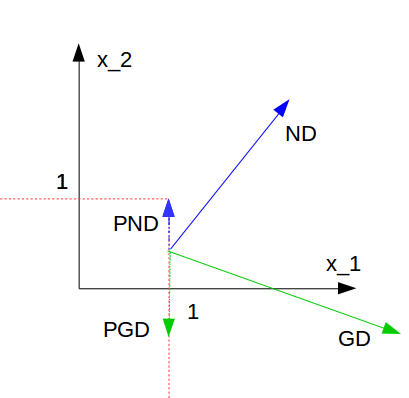
\includegraphics[width=0.7\linewidth]{example7}
	\caption[Newton and gradient direction]{Blue arrows are Newton directions (projected and not), while green ones are gradient directions (projected and not). We see how the projected Newton direction (PND) is increasing for the norm of $ F $ since it lies in the semi-plane in which the function is supposed to grow, that is the semi-plane that has the opposite of GD. Instead, the projection of gradient direction (PGD) is in the decreasing semi-plane.}
	\label{esempio7}
\end{figure}

\subsubsection{Numerical example}
In addiction to the analytical example that we have just shown, there is also a numerical one in \cite{MAIN} (Example 8), whose aim is to show the performances of the new projected Newton-Krylov method. It is about a system of nonlinear equations for $ \textbf{x} = (x_1, \dots, x_n)^T $ with $ \Omega = \{ \textbf{x} \in \mathbb{R}^n | x_1 \in [0.8, 2], x_i \in [0.5, 2], 2 \leq i \leq n \} $. The system is
\begin{equation*}
\begin{cases}
x_1^2 - 1 = 0,\\
x_1 - x_2^3 = 0,\\
x_2 - x_3^3 = 0, \\
\; \;  \; \; \vdots \\
x_{n-2} - x_{n-1}^2 = 0,\\ 
x_{n-1} - x_n = 0
\end{cases}
\end{equation*}
with solution  $ \textbf{x}^* = (1, \dots, 1)^T $ in $ \Omega $.\\ 
As a first approach, we tried to implement this problem by our self with $ n = 100 $ in order to compare our results with the ones of the paper. The information that we had about settings of Algorithm \ref{pNK}, was the following: 
\begin{enumerate}[label=(\alph*)]
	\item initial guess for the nonlinear iterations $ \textbf{x}_0 (1:20) = 0.9  $ and $ \textbf{x}_0 (21:100) = 0.5$, and zero vector for the linear ones;
	\item termination tolerance rule for nonlinear iteration: $ ||F(\textbf{x}_k)|| \leq 10^{-12} $;
	\item choice of linear search parameter $ \lambda = \lambda_0^ m$, with $ \lambda_0 = 0.5 $ for porjected Newton direction and $ \lambda_0 = 0.8 $ for projected gradient one.
	\item $ \sigma = t = 10^{-4} $, $ m_{max} = 20 $, $ \eta_{max} = 0.9 $;
	\item linear solver GMRES.
\end{enumerate}
For the choice of forcing term $ \eta_k $ the authors just say that they used one of the options in \cite{Forcingterm}, the ones that we illustrated in the previous chapter. The problem for us was that we did not know exactly which one was the choice used and which was the value of the parameters. Using all information we had and the values of residual norm $ ||F(\textbf{x})|| $ that we should have obtained (table in Figure \ref{results_example8}), we applied a reverse iterative technique to find out the forcing terms. In practice, we interpolated the tolerance needed in the linear solver (so the forcing term) to arrive to the residual norms of Figure \ref{results_example8} and, after few steps, we found that they used Choice 2 \eqref{Choice2} with $ \alpha = 2 $, $ \gamma = 0.9 $ and $ \eta_0 \simeq 0.765518 $.\\
\begin{figure}[h]
	\centering
	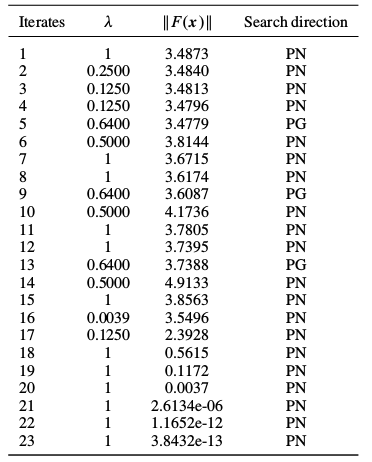
\includegraphics[width=0.6\linewidth]{results_example8}
	\caption[Table of results of example 8 in \cite{MAIN}]{Table of results of Example 8 in \cite{MAIN}, PN indicates that it was used projected Newton direction and PG projected gradient direction. The values of columns of $ \lambda $ and $ ||F(\textbf{x})|| $ are shifted by one respect to the others; indeed, for example, the norm of $ F $, that was achieved in iteration 1, and the $ \lambda $, that was used, are the ones in the second row.}
	\label{results_example8}
\end{figure}
First of all, we have to point out that in Figure \ref{results_example8}, each value of $ ||F(\textbf{x})|| $ is actually the input value of that iteration, so, for example, $ 3.4873 $ corresponds to $ ||F(\textbf{x}_0)|| $, and the value in the second iteration is the residual norm that comes from the first iteration. The same is true for values of $ \lambda $ , so the columns of $ \lambda $ and $ ||F(\textbf{x})|| $ are shifted by one iteration respect to the other two columns.\\
After all this procedure, we realized that the values of $ \lambda $ in iterate 5 and 6 are reported wrongly, indeed in 5, $ \lambda $ is equal actually to $ 0.5^2 $ and not to $ 0.8^2 $ because it refers to the previous step that uses PN, and not PG. Indeed in 6, $ \lambda$ is equal to $0.8 $ and not to $ 0.5 $ for the same reason. This correction needs to be done for iterates 9, 10, 13 and 14 as well. We have reported our results in Figure \ref{our_example8} in the same format as in Figure \ref{res_paper}.\\
Another thing that we noticed, more important, was that, in order to have the same results as in the paper's Table, we had to force $ \lambda $ to be equal to $ 0.8 $ in each time PG was used, even if \eqref{ineqPG} was not verified. When we did the test as Algorithm \ref{pNK} indicates, at iteration 5, $ \lambda = 0.8 $ was not enough, so the algorithm selected $ \lambda = 0.8^4 $ to satisfy \eqref{ineqPG}. Therefore, all the convergence behavior, that follows step 5, changes. Figure \ref{res_paper} and \ref{res_our}, shown their and our trend of the residual norm.\\
\begin{figure}[h]
	\centering
	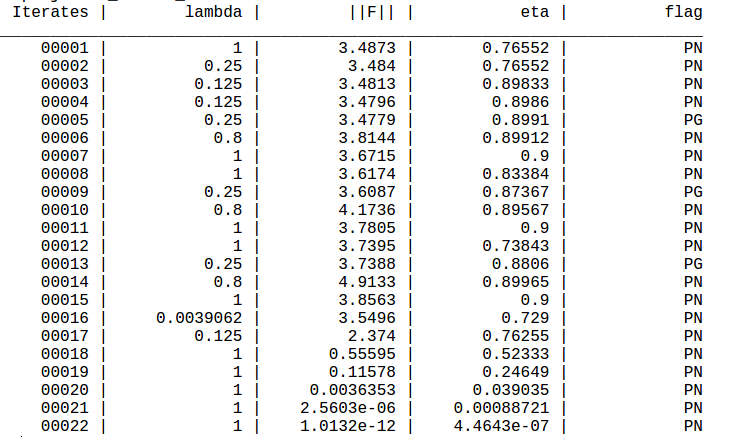
\includegraphics[width=1\linewidth]{ourresults8}
	\caption[Table of our results for example 8 in \cite{MAIN}]{Table of our results for Example 8 in \cite{MAIN}. We managed to generate this results, that are equal to the ones in Figure \ref{results_example8}, at least in the first 16 iterations, with a revers iterative technique that found missed information, that is the choice for $ \eta_k $. But we had also to impose $ \lambda = 0.8 $ in each PG step, even if the inequality \eqref{ineqPG} was not satisfied.}
	\label{our_example8}
\end{figure}
\begin{figure}[h]
	\centering
	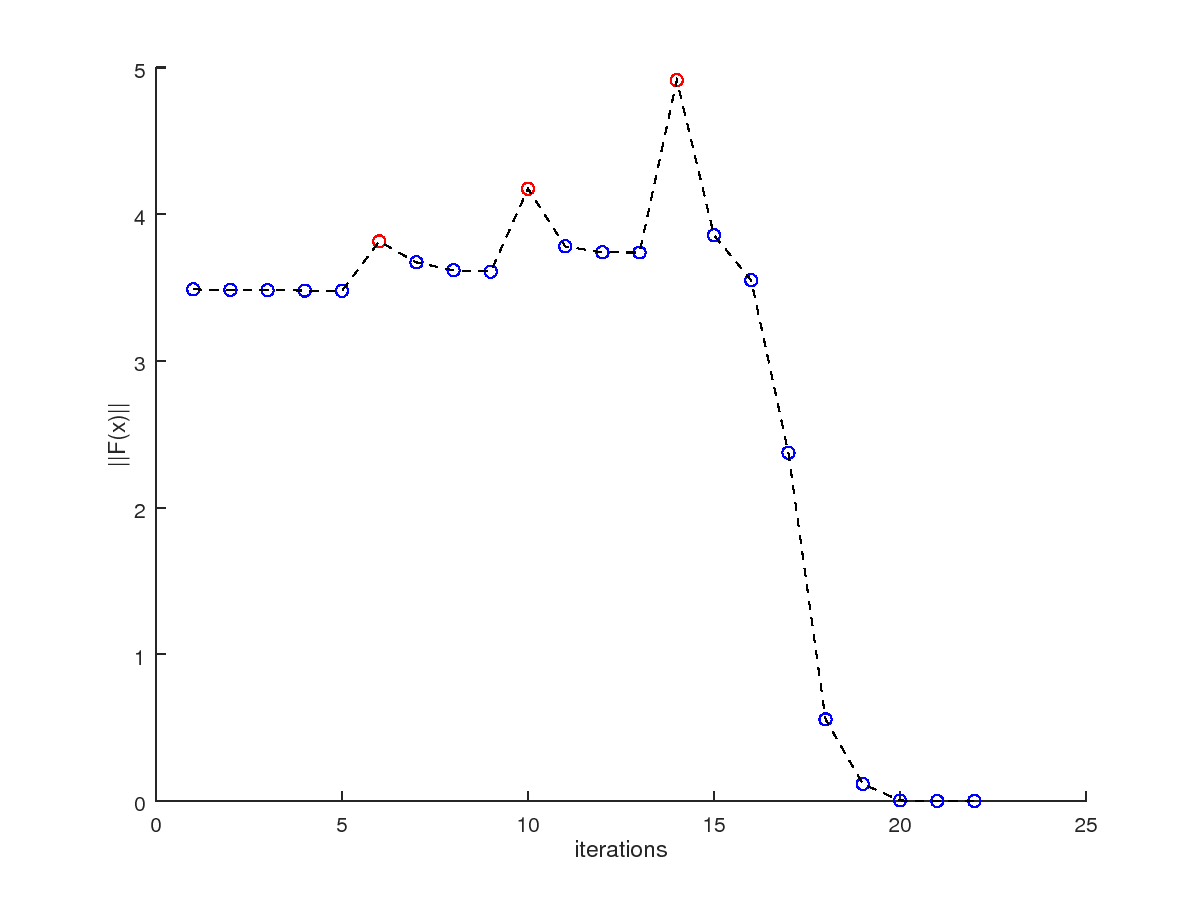
\includegraphics[width=0.8\linewidth]{res_paper}
	\caption[Plot of residuals found in \cite{MAIN}]{Residual norms according to paper's result, blu point are PN and red ones are PG. We see that they does not respect the main characteristic of the analyzed method, which is that the norm of $ F $ has not to increase. This happens because inequality \eqref{ineqPG} is not satisfied.}
	\label{res_paper}
\end{figure}
\begin{figure}[h]
	\centering
	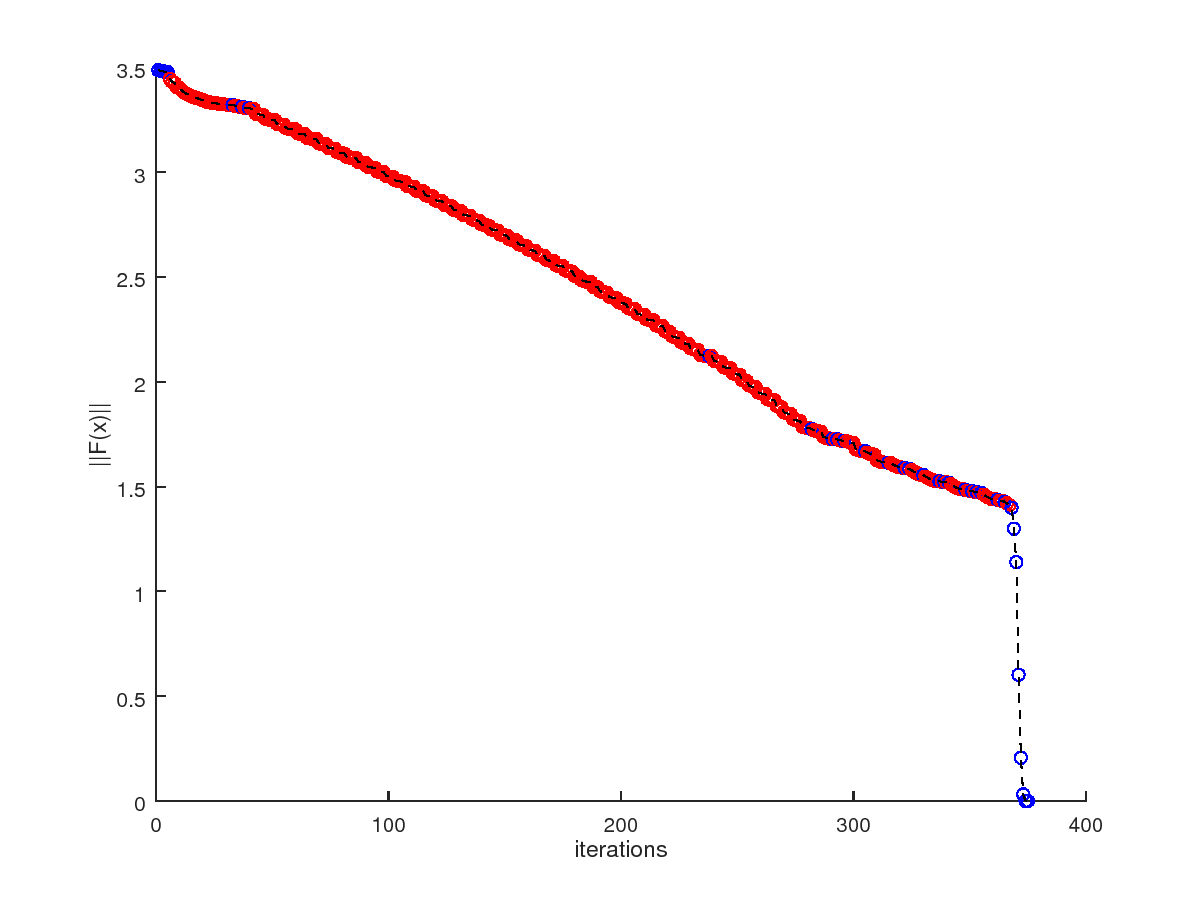
\includegraphics[width=0.8\linewidth]{res_our}
	\caption[Plot of residuals found by us]{Residual norms that we obtained implementing Algorithm \ref{pNK} in the right way. In this case the number of iterations is much bigger than the one promised in the paper and a lot of PG are used, reason for which the convergence is slow. However, without the use of PG, it does not converge, because at each step Newton direction tries to push in the direction of the solution out of $ \Omega $, that is $ \textbf{x} =(-1, -1, \dots, -1 )^T  $, but the result is always projected on the constraints. That brief analysis predicts a quite slow method, but at least robust. }
	\label{res_our}
\end{figure}
Actually, there was no need to implement all by our self to see that there is something wrong. In fact, if we notice the trend of the residual norm in Figure \ref{results_example8} and \ref{res_paper}, we realize that is not non-increasing. That should not happen when \eqref{ineqPG} is verified, since $ \sigma $ has to be positive and $\nabla \Theta(\textbf{x}_k)^T (\mathcal{P}(\textbf{x}_k + \lambda \textbf{d}_k)- \textbf{x}_k)  $ has to be negative because the projected gradient direction is a descent one (Lemma \ref{lem_descent}). So the residual norm has to be strictly decreasing. \\
We have discovered that in our implementation much more iterations were required to reach convergence and for most of them it is used projected gradient direction, so the decrease of residual norm is very slow. Indeed the use of PG cannot be considered as a massive one because it is too slow, it should intervene in isolated steps when PN is not able to find a acceptable direction. \\
In any case, we tried to implement the algorithm without PG and we verified that it is not going to converge because the PN forces $\textbf{x} $ to arrive to the other solution $ \textbf{x}^* = (-1, \dots, -1)^T$, that is out of $ \Omega $, so $ \textbf{x} + \lambda \textbf{d} $ is always projected on the constraints, consequently the algorithm remains stuck. Figure \ref{res_our} predicts a quite slow method, but at least robust, because it manage to converge to the domain's solution. 


%\include{conclusioni}





\appendix %---------------

%\include{appendiceA}


\backmatter %--------------
%\phantomsection 
\addcontentsline{toc}{chapter}{Bibliography}
\bibliographystyle{plain}
\bibliography{bibliografia}


\end{document}